%%%%%%%%%%%%%%%%%%%%%%%%%%%%%%%%%%%%%%%%%%%%%%%%%%%%%%%%%%%%%%%%%%%%%
%% This is a (brief) model paper using the achemso class
%% The document class accepts keyval options, which should include
%% the target journal and optionally the manuscript type.
%%%%%%%%%%%%%%%%%%%%%%%%%%%%%%%%%%%%%%%%%%%%%%%%%%%%%%%%%%%%%%%%%%%%%
\documentclass[journal=jacsat,manuscript=article]{achemso}

%%%%%%%%%%%%%%%%%%%%%%%%%%%%%%%%%%%%%%%%%%%%%%%%%%%%%%%%%%%%%%%%%%%%%
%% Place any additional packages needed here.  Only include packages
%% which are essential, to avoid problems later. Do NOT use any
%% packages which require e-TeX (for example etoolbox): the e-TeX
%% extensions are not currently available on the ACS conversion
%% servers.
%%%%%%%%%%%%%%%%%%%%%%%%%%%%%%%%%%%%%%%%%%%%%%%%%%%%%%%%%%%%%%%%%%%%%
\usepackage[version=3]{mhchem} % Formula subscripts using \ce{}

%%%%%%%%%%%%%%%%%%%%%%%%%%%%%%%%%%%%%%%%%%%%%%%%%%%%%%%%%%%%%%%%%%%%%
%% If issues arise when submitting your manuscript, you may want to
%% un-comment the next line.  This provides information on the
%% version of every file you have used.
%%%%%%%%%%%%%%%%%%%%%%%%%%%%%%%%%%%%%%%%%%%%%%%%%%%%%%%%%%%%%%%%%%%%%
%%\listfiles

%%%%%%%%%%%%%%%%%%%%%%%%%%%%%%%%%%%%%%%%%%%%%%%%%%%%%%%%%%%%%%%%%%%%%
%% Place any additional macros here.  Please use \newcommand* where
%% possible, and avoid layout-changing macros (which are not used
%% when typesetting).
%%%%%%%%%%%%%%%%%%%%%%%%%%%%%%%%%%%%%%%%%%%%%%%%%%%%%%%%%%%%%%%%%%%%%
\newcommand*\mycommand[1]{\texttt{\emph{#1}}}

%%%%%%%%%%%%%%%%%%%%%%%%%%%%%%%%%%%%%%%%%%%%%%%%%%%%%%%%%%%%%%%%%%%%%
%% Meta-data block
%% ---------------
%% Each author should be given as a separate \author command.
%%
%% Corresponding authors should have an e-mail given after the author
%% name as an \email command. Phone and fax numbers can be given
%% using \phone and \fax, respectively; this information is optional.
%%
%% The affiliation of authors is given after the authors; each
%% \affiliation command applies to all preceding authors not already
%% assigned an affiliation.
%%
%% The affiliation takes an option argument for the short name.  This
%% will typically be something like "University of Somewhere".
%%
%% The \altaffiliation macro should be used for new address, etc.
%% On the other hand, \alsoaffiliation is used on a per author basis
%% when authors are associated with multiple institutions.
%%%%%%%%%%%%%%%%%%%%%%%%%%%%%%%%%%%%%%%%%%%%%%%%%%%%%%%%%%%%%%%%%%%%%
\author{Hongjian Li}
\email{jackyleehongjian@gmail.com}
\author{Kwong-Sak Leung}
\author{Man-Hon Wong}
\affiliation[Chinese University of Hong Kong]
{Department of Computer Science and Engineering, Chinese University of Hong Kong, Shatin, New Territories, Hong Kong}
\author{Pedro J. Ballester}
%\email{pedro.ballester@ebi.ac.uk}
\affiliation[European Bioinformatics Institute]
{European Bioinformatics Institute, Wellcome Trust Genome Campus, Hinxton, Cambridge - CB10 1SD, UK}

%%%%%%%%%%%%%%%%%%%%%%%%%%%%%%%%%%%%%%%%%%%%%%%%%%%%%%%%%%%%%%%%%%%%%
%% The document title should be given as usual. Some journals require
%% a running title from the author: this should be supplied as an
%% optional argument to \title.
%%%%%%%%%%%%%%%%%%%%%%%%%%%%%%%%%%%%%%%%%%%%%%%%%%%%%%%%%%%%%%%%%%%%%
\title[RF::Cyscore]{Substituting Random Forest for Multiple Linear Regression Improves Binding Affinity Prediction Performance of Empirical Scoring Functions: Cyscore as a Case Study}

%%%%%%%%%%%%%%%%%%%%%%%%%%%%%%%%%%%%%%%%%%%%%%%%%%%%%%%%%%%%%%%%%%%%%
%% Some journals require a list of abbreviations or keywords to be
%% supplied. These should be set up here, and will be printed after
%% the title and author information, if needed.
%%%%%%%%%%%%%%%%%%%%%%%%%%%%%%%%%%%%%%%%%%%%%%%%%%%%%%%%%%%%%%%%%%%%%
\abbreviations{MLR,RF}
\keywords{Molecular docking, binding affinity, drug discovery, machine learning}

%%%%%%%%%%%%%%%%%%%%%%%%%%%%%%%%%%%%%%%%%%%%%%%%%%%%%%%%%%%%%%%%%%%%%
%% The manuscript does not need to include \maketitle, which is
%% executed automatically.
%%%%%%%%%%%%%%%%%%%%%%%%%%%%%%%%%%%%%%%%%%%%%%%%%%%%%%%%%%%%%%%%%%%%%
\begin{document}

%%%%%%%%%%%%%%%%%%%%%%%%%%%%%%%%%%%%%%%%%%%%%%%%%%%%%%%%%%%%%%%%%%%%%
%% The "tocentry" environment can be used to create an entry for the
%% graphical table of contents. It is given here as some journals
%% require that it is printed as part of the abstract page. It will
%% be automatically moved as appropriate.
%%%%%%%%%%%%%%%%%%%%%%%%%%%%%%%%%%%%%%%%%%%%%%%%%%%%%%%%%%%%%%%%%%%%%
\begin{tocentry}

Some journals require a graphical entry for the Table of Contents.
This should be laid out ``print ready'' so that the sizing of the
text is correct.

Inside the \texttt{tocentry} environment, the font used is Helvetica
8\,pt, as required by \emph{Journal of the American Chemical
Society}.

The surrounding frame is 9\,cm by 3.5\,cm, which is the maximum
permitted for  \emph{Journal of the American Chemical Society}
graphical table of content entries. The box will not resize if the
content is too big: instead it will overflow the edge of the box.

This box and the associated title will always be printed on a
separate page at the end of the document.

\end{tocentry}

%%%%%%%%%%%%%%%%%%%%%%%%%%%%%%%%%%%%%%%%%%%%%%%%%%%%%%%%%%%%%%%%%%%%%
%% The abstract environment will automatically gobble the contents
%% if an abstract is not used by the target journal.
%%%%%%%%%%%%%%%%%%%%%%%%%%%%%%%%%%%%%%%%%%%%%%%%%%%%%%%%%%%%%%%%%%%%%
\begin{abstract}

State-of-the-art protein-ligand docking methods are generally limited by the traditionally low accuracy of their scoring functions, which are used to predict binding affinity and thus vital for discriminating between active and inactive compounds. Despite intensive research in recent years, many newly-developed scoring functions hardly show satisfactory prediction performance. They often assume a predetermined additive functional form for some sophisticated numerical features, and use standard least squares multivariate linear regression on experimental data to derive the coefficients. In this study we show that such a simple functional form is detrimental for its performance, and replacing linear regression by machine learning techniques like random forest (RF) can significantly improve prediction performance. We investigate the conditions of applying RF under various contexts and find that RF requires sufficient structural features and training samples to implicitly and comprehensively capture the non-linearity between structural features and measured binding affinities. The future availability of more and more resolved structures will continue to enlarge the performance gap between empirical and RF-based scoring functions. Lastly, we show that RF-based scoring functions can be as interpretable as empirical ones via proper estimation of feature importance. We use Cyscore, an empirical scoring function recently published in a top journal, as a baseline for comparison study.

\end{abstract}

%%%%%%%%%%%%%%%%%%%%%%%%%%%%%%%%%%%%%%%%%%%%%%%%%%%%%%%%%%%%%%%%%%%%%
%% Start the main part of the manuscript here.
%%%%%%%%%%%%%%%%%%%%%%%%%%%%%%%%%%%%%%%%%%%%%%%%%%%%%%%%%%%%%%%%%%%%%
\section{Introduction}

Protein-ligand docking is a computational tool that predicts how a ligand binds to a target protein and their binding affinity. Hence docking is useful in elaborating intermolecular interactions and enhancing the potency and selectivity of binding in subsequent phases of computer-aided drug design. Docking has a wide variety of pragmatic and successful applications in structure-based virtual screening \cite{1383}, drug repurposing \cite{1384}, lead compound optimization \cite{1385}, protein cavity identification \cite{1217}, and protein function prediction \cite{1386}.

Docking consists of two major operations: predicting the position, orientation and conformation of a ligand when docked to the protein's binding pocket, and predicting their binding strength. The former operation is known as pose generation, and the latter is known as scoring. State-of-the-art docking methods, such as AutoDock Vina \cite{595} and idock \cite{1153}, work reasonably well at pose generation with a redocking success rate of over 50\% \cite{1362} on the benchmarks of both PDBbind v2012 and v2011 \cite{529,530} and the CSAR NRC HiQ Set 24Sept2010 \cite{857,960}. However, the single most critical limitation of docking is the traditionally low accuracy of the scoring functions.

Empirical scoring functions assume a fixed functional form for the relationship between the numerical features that characterize the protein-ligand complex and its predicted binding affinity. Such a functional form is composed of the energetic contributions of various intermolecular interactions, and is often additive. The overall binding affinity is calculated as a weighted sum of several physically meaningful terms, while their coefficients are typically derived from standard least squares multivariate linear regression (MLR) on experimental data. Cyscore \cite{1372}, a recently published scoring function, is an example of empirical scoring functions.

Cyscore assumes that the overall protein-ligand binding free energy can be decomposed into four terms: hydrophobic free energy, van der Waals interaction energy, hydrogen bond interaction energy and ligand's conformational entropy. Cyscore focuses on improving the prediction of hydrophobic free energy by using a novel curvature-dependent surface-area model, which was claimed to be able to distinguish convex, planar and concave surface in hydrophobic free energy calculation.

In addition to empirical scoring functions, recent years have seen a growing number of new developments of machine-learning scoring functions (see \cite{1373} for a brief review), with RF-Score \cite{564} being the first that introduced a large improvement over classical approaches. RF-Score, as its name suggests, uses Random Forest (RF) \cite{1309} to implicitly learn the functional form in an entirely data-driven manner, and thus circumvents the modelling assumption imposed by empirical scoring functions. RF-Score was shown to significantly outperform 16 classical scoring functions when evaluated on the common PDBbind v2007 benchmark \cite{564}. Despite being a recent development, RF-Score has already been successfully used to discover a large number of innovative binders against antibacterial DHQase2 targets \cite{1281}. For the purpose of prospective virtual screening, RF-Score has now been incorporated into istar \cite{1362}, our large-scale docking service available at http://istar.cse.cuhk.edu.hk/idock.

In this study we compare the prediction performance of two regression models MLR and RF, and investigate their application conditions and interpretability under various contexts. The Methods section introduces MLR and RF, three sets of features, three benchmarks, and four performance metrics. The Results section analyzes the prediction performance of MLR and RF on the three benchmarks and discusses the conditions of applying MLR and RF. The Conclusions section emphasizes the importance of abundance of features and samples for training RF.

\section{Methods}

\subsection{Multiple Linear Regression (MLR) with Cyscore features}

Cyscore is a empirical scoring function in an additive functional form of four terms (Eq. \ref{eqn:cyscore}), whose coefficients were obtained by MLR on 247 high-quality complexes carefully selected from PDBbind v2012 refined set. The intercept value was not reported in the original publication, but was included in this study in order to compute absolute binding affinity values. We use MLR::Cyscore to denote the scoring function built with MLR and the 4 features from Cyscore. It is noteworthy that Cyscore is a pure MLR model, unlike AutoDock Vina \cite{595} which is a quasi MLR model because the number of rotatable bonds $N_{rot}$ is in the denominator so as to penalize ligand flexibility (see \cite{1362} for the exact equation) and therefore MLR::Vina requires an additional grid search for the weight of the $N_{rot}$ parameter. So this study allows a more direct comparison between MLR and RF.

\begin{equation}
\Delta G_{bind} = k_h\Delta G_{hydrophobic} + k_v\Delta G_{vdw} + k_b\Delta G_{hbond} + k_e\Delta G_{entropy} + C
\label{eqn:cyscore}
\end{equation}

\subsection{Random Forest (RF) with Cyscore, AutoDock Vina and RF-Score features}

A RF \cite{1309} is a consensus of a large number of different decision trees generated from random bootstrap sampling of the same training data. During tree construction, at each inner node RF chooses the best splitting feature that results in the highest purity gain from a normally small number (mtry) of randomly selected features rather than utilizing all input features. In regression problems, the final output is calculated as the arithmetic mean of all individual tree predictions in the RF. Further details on RF construction can be found in \cite{564,1362}.

In this study, multiple RFs of the default number of 500 trees were built using values of the mtry control parameter from one to the total number of input features. The selected RF was the one resulting in the lowest root mean square error (RMSE) on the Out-of-Bag (OOB) samples of the training set. Only one single random seed was used because seed is not a significant impact factor of the prediction performance, and using fewer seeds has the additional advantage of leading to computationally faster training process.

In our experiments we aimed at analyzing how RF responds to varying numbers of features and hence we selected three sets of features: Cyscore \cite{1372}, AutoDock Vina \cite{595} and RF-Score \cite{564}. Cyscore comprises four numerical features: $\Delta G_{hydrophobic}$, $\Delta G_{vdw}$, $\Delta G_{hbond}$ and $\Delta G_{entropy}$. AutoDock Vina comprises six numerical features: $Gauss_1$, $Gauss_2$, $Repulsion$, $Hydrophobic$, $HBonding$ and $N_{rot}$. RF-Score comprises 36 features, defined as the occurrence count of intermolecular contacts between two elemental atom types. Four atom types for proteins (C, N, O, S) and nine for ligands (C, N, O, S, P, F, Cl, Br, I) were selected so as to generate dense features while considering all the heavy atom types commonly observed in protein-ligand complexes. Table \ref{tbl:features} summarizes the three combinations of these feature sets used to train RF models. Altogether four models (MLR::Cyscore, RF::Cyscore, RF::CyscoreVina and RF::CyscoreVinaElem) were evaluated in this study.

\begin{table}[h]
\caption{The three combinations of three different sets of features used to train RF models in this study.}
\label{tbl:features}
\begin{tabular}{ll}
\hline
model & features\\
\hline
RF::Cyscore         & 4 Cyscore features\\
RF::CyscoreVina     & 4 Cyscore features + 6 AutoDock Vina features\\
RF::CyscoreVinaElem & 4 Cyscore features + 6 AutoDock Vina features + 36 RF-Score features\\
\hline
\end{tabular}
\end{table}

\subsection{PDBbind v2007 and v2012 benchmarks}

The PDBbind benchmark is arguably the most widely used for binding affinity prediction. It contains an especially diverse collection of experimentally resolved protein-ligand complexes, assembled through a systematic mining of the yearly releases of the entire PDB \cite{540,537}. For each complex, the experimentally measured binding affinity, either dissociation constant Kd or inhibition constant Ki, was manually collected from its primary literature reference. The complexes with a resolution of 2.5\AA\ or better and with the ligand comprising merely nine common heavy atom types (C, N, O, F, P, S, Cl, Br, I) were filtered to constitute the refined set. These complexes were then clustered by protein sequence similarity with a cutoff of 90\%, and for each of the resulting clusters with at least five complexes, the three complexes with the highest, median and lowest binding affinity were selected to constitute the core set.

On one hand, Cyscore was tested on two independent sets: PDBbind v2007 core set (N=195) and PDBbind v2012 core set (N=201). The experimental binding affinities span 12.56 and 9.85 pKd units in the former and latter test sets, respectively. On the other hand, Cyscore was trained on a special set of 247 complexes carefully selected from the PDBbind v2012 refined set using certain criteria \cite{1372} (e.g. structural resolution < 1.8\AA, binding affinity spans 1 to 11 kcal/mol, protein sequence similarity and ligand chemical composition are different from the test set), ensuring that the training complexes are of high quality and do not overlap with any of the two test sets. In this study we used exactly the same training set and the same test sets in order to make a fair comparison to Cyscore.

Furthermore, considering the fact that 16 classical scoring functions have already been evaluated \cite{1313} on PDBbind v2007 core set and the top performing of them (e.g. X-Score) were trained on the remaining 1105 complexes in PDBbind v2007 refined set, we also used these 1105 complexes as another training set to permit a direct comparison. Using predefined training and test sets, where other scoring functions had previously been trained and tested, has the advantage of reducing the risk of using a benchmark complementary to one particular scoring function.

Likewise for the PDBbind v2012 benchmark, we used an additional training set comprising the complexes in PDBbind v2012 refined set excluding those in PDBbind v2012 core set. This led to a total of 2696 complexes. By construction, this training set does not overlap with the test set. % TODO: motivate why three sets (core07,core12,ref13\ref12) and say something about bias in using core07 and core12.

\subsection{PDBbind v2013 benchmark}

We propose a new benchmark to investigate how prediction performance of the four models changes in cross validation and with varying numbers of training samples. We used PDBbind v2013 refined set (N=2959), which is the latest version up to date and comprises the most comprehensive structural data.

We used 5-fold cross validation, as was used by the recently-published empirical scoring function ID-Score \cite{1305}, to overcome the overfitting problem and minimize generalization errors. The entire PDBbind v2013 refined set (N=2959) was divided into five equal partitions using uniform sampling on a round-robin basis: the entire 2959 complexes were first sorted in the ascending order of their measured binding affinity, and the complexes with the 1st, 6th, 11th, etc. lowest binding affinity belonged to the first partition, the complexes with the 2nd, 7th, 12th, etc. lowest binding affinity belonged to the second partition, and so on. This partitioning method, though not completely random, has two advantages: on one hand, each partition is guaranteed to span the largest range of binding affinities and incorporates the largest structural diversity of different protein families; on the other hand, each partition is composed of a deterministic list of complexes, ensuring reproducibility and comparisons in future studies. Table \ref{tbl:partitions} summarizes the statistics of the five partitions. The PDB IDs and measured binding affinities of the complexes in the five partitions are available in the supporting file cv.xlsx.

\begin{table}
\caption{The statistics of the five partitions of PDBbind v2013 refined set (N=2959).}
\label{tbl:partitions}
\begin{tabular}{rrrr}
\hline
\# & complexes & lowest pKd & highest pKd\\
\hline
1 & 592 & 2.00 & 11.74\\
2 & 592 & 2.00 & 11.80\\
3 & 592 & 2.00 & 11.85\\
4 & 592 & 2.00 & 11.92\\
5 & 591 & 2.05 & 11.72\\
\hline
\end{tabular}
\end{table}

We then used the partition on which the best performance was obtained (It turned out to be partition 2 (N=592). See the Results section.) as the test set in PDBbind v2013 benchmark, and used the remaining four partitions (1, 3, 4, 5) to construct four training sets of incremental sizes: the first training set comprises partition 1 (N=592), the second training set comprises partitions 1 and 3 (N=1184), the third training set comprises partitions 1, 3 and 4 (N=1776), and the fourth training set comprises partitions 1, 3, 4 and 5 (N=2367). Therefore this new benchmark provides a way to study how prediction performance varies with training sample size, and its test set has a significantly larger number of complexes (N=592) compared to PDBbind v2007 (N=195) and v2012 (N=201) benchmarks.

Table \ref{tbl:benchmarks} summarizes the numbers of test samples and training samples for each of the three benchmarks.

\begin{table}
\caption{The numbers of test samples and training samples for the PDBbind v2007, v2012 and v2013 benchmarks used in this study.}
\label{tbl:benchmarks}
\begin{tabular}{rrr}
\hline
benchmark & test samples & training samples\\
\hline
v2007 & 195 &  247\\
v2007 & 195 & 1105\\
v2012 & 201 &  247\\
v2012 & 201 & 2696\\
v2013 & 592 &  592\\
v2013 & 592 & 1184\\
v2013 & 592 & 1776\\
v2013 & 592 & 2367\\
\hline
\end{tabular}
\end{table}

\subsection{Performance metrics}

Prediction performance was quantified through standard deviation SD in linear correlation, Pearson correlation coefficient Rp and Spearman correlation coefficient Rs between the measured and predicted binding affinities of the test set. These three metrics are commonly used in the community \cite{1313}, and the SD metric is essentially the same as the residual standard error (RSE) metric used in some other studies \cite{963}.

The above three metrics are invariant under linear transformations (e.g. changing the intercept or coefficient values in Eq. \ref{eqn:cyscore} affects none of these metrics), so they are mainly used for comparative purpose. In some applications, however, the ultimate goal of scoring functions is to report an absolute binding affinity value as close to the measured value as possible. Hence we use a more realistic metric, the root mean square error RMSE between measured and predicted binding affinities without a linear correlation on the test set.

Mathematically, equations \ref{eqn:rmse}, \ref{eqn:sdev}, \ref{eqn:pcor} and \ref{eqn:scor} show the exact expressions of the four metrics. Given a scoring function $f$ and the features $\overrightarrow{x}^{(n)}$ describing the $n$th complex out of $N$ complexes in the test set, $p^{(n)}=f(\overrightarrow{x}^{(n)})$ is the predicted binding affinity, $\{\hat{p}^{(n)}\}$ are the fitted values from the linear model between $\{y^{(n)}\}$ and $\{p^{(n)}\}$ on the test set, whereas $\{y_r^{(n)}\}$ and $\{p_r^{(n)}\}$ are the rankings of $\{y^{(n)}\}$ and $\{p^{(n)}\}$, respectively. Lower values in RMSE and SD and higher values in Rp and Rs indicate better prediction performance.

\begin{equation}
RMSE = \sqrt{\frac{1}{N}\sum_{n=1}^N(p^{(n)}-y^{(n)})^2}
\label{eqn:rmse}
\end{equation}

\begin{equation}
SD = \sqrt{\frac{1}{N-2}\sum_{n=1}^N(\hat{p}^{(n)}-y^{(n)})^2}
\label{eqn:sdev}
\end{equation}

\begin{equation}
R_p = \frac{N\sum_{n=1}^Np^{(n)}y^{(n)}-\sum_{n=1}^Np^{(n)}\sum_{n=1}^Ny^{(n)}}{\sqrt{(N\sum_{n=1}^N(p^{(n)})^2-(\sum_{n=1}^Np^{(n)})^2)(N\sum_{n=1}^N(y^{(n)})^2-(\sum_{n=1}^Ny^{(n)})^2)}}
\label{eqn:pcor}
\end{equation}

\begin{equation}
R_s = \frac{N\sum_{n=1}^Np_r^{(n)}y_r^{(n)}-\sum_{n=1}^Np_r^{(n)}\sum_{n=1}^Ny_r^{(n)}}{\sqrt{(N\sum_{n=1}^N(p_r^{(n)})^2-(\sum_{n=1}^Np_r^{(n)})^2)(N\sum_{n=1}^N(y_r^{(n)})^2-(\sum_{n=1}^Ny_r^{(n)})^2)}}
\label{eqn:scor}
\end{equation}

\section{Results and discussion}

Figure \ref{fig:stat} plots the prediction performance of MLR and RF using different numbers of features and training samples on PDBbind v2007 benchmark (N=195), PDBbind v2012 benchmark (N=201) and PDBbind v2013 benchmark (N=592).

\begin{figure}[ht!]
\minipage{0.30\textwidth}
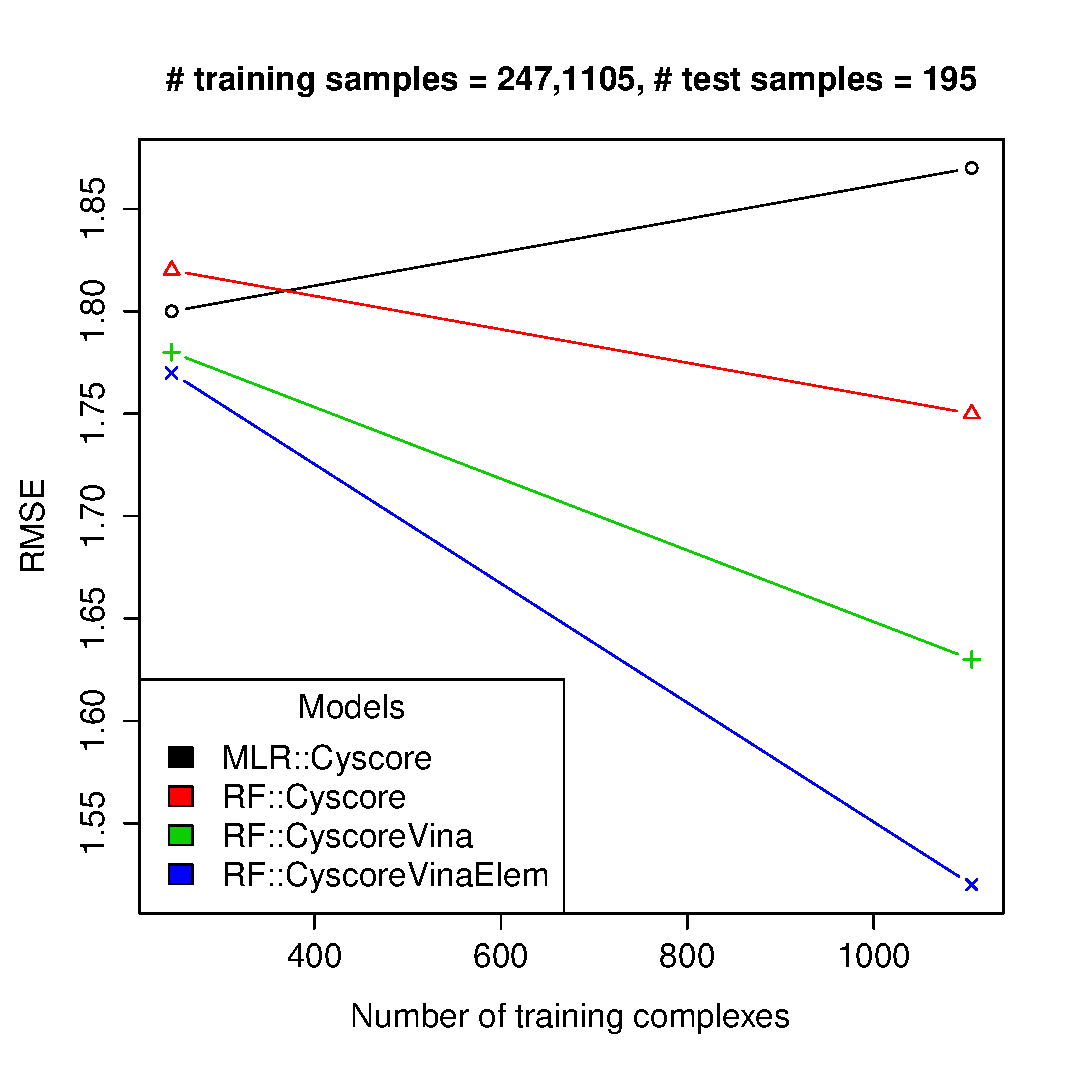
\includegraphics[width=\linewidth]{../rfcyscore/tst-195-rmse.eps}
\endminipage
\minipage{0.30\textwidth}
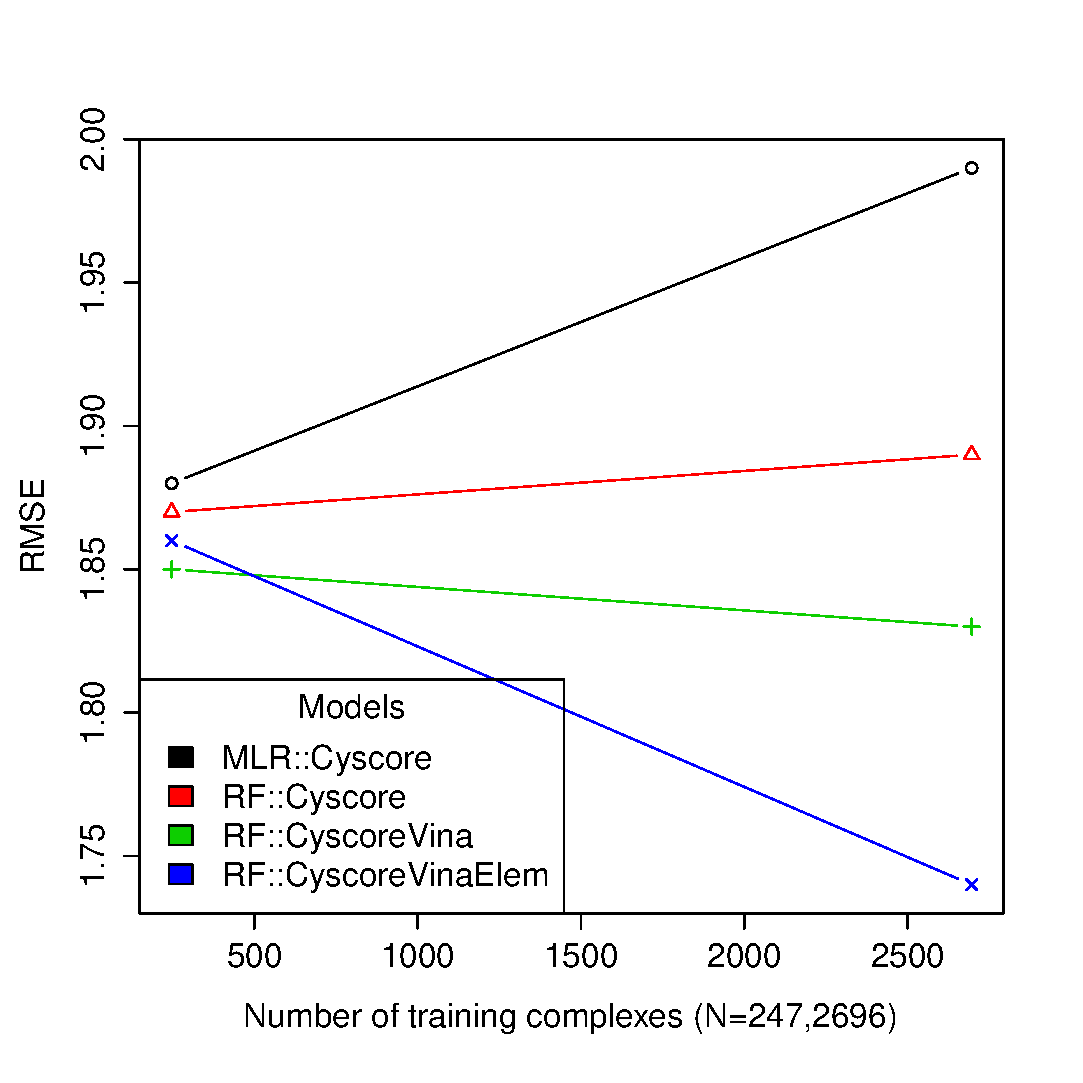
\includegraphics[width=\linewidth]{../rfcyscore/tst-201-rmse.eps}
\endminipage
\minipage{0.30\textwidth}
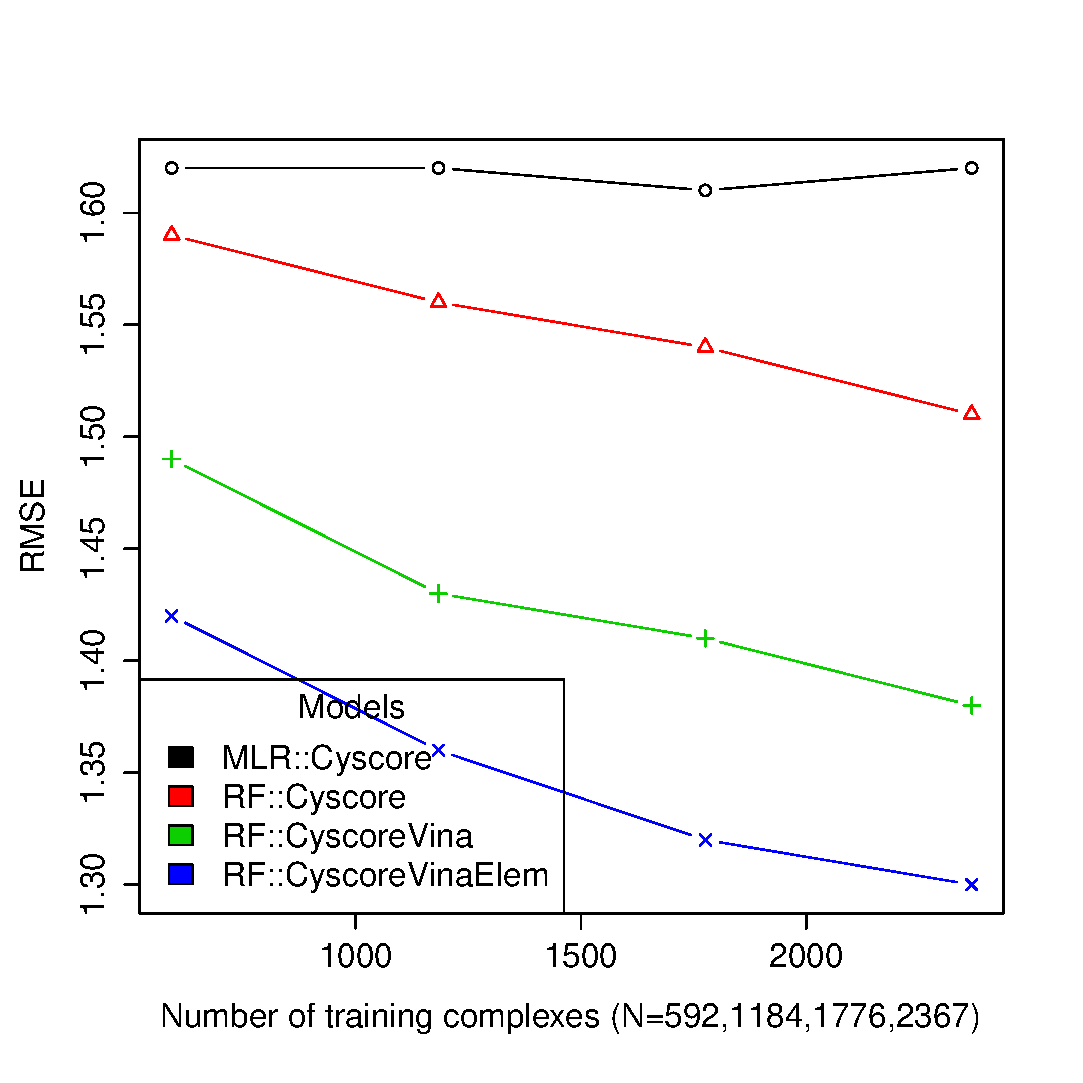
\includegraphics[width=\linewidth]{../rfcyscore/tst-592-rmse.eps}
\endminipage
\\
\minipage{0.30\textwidth}
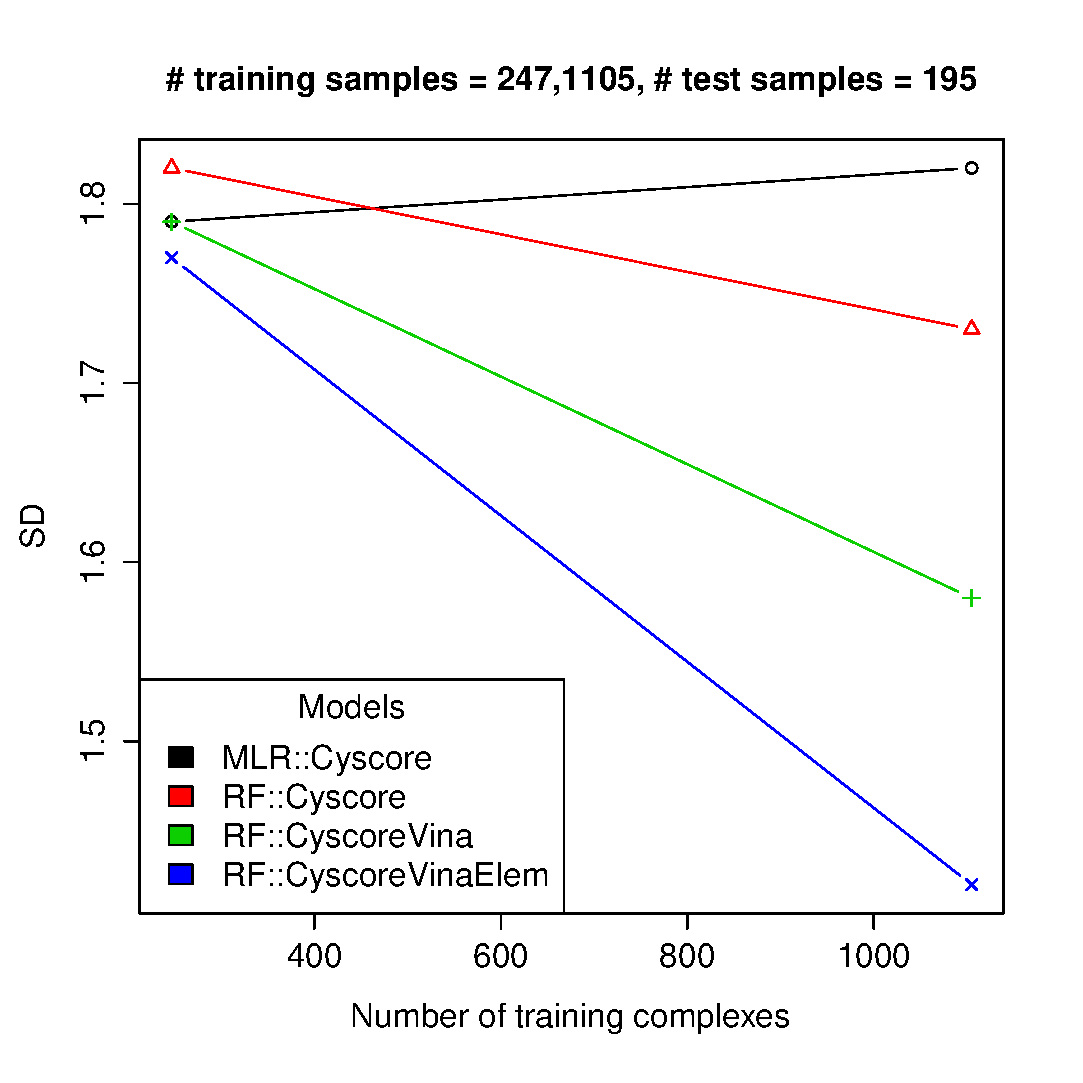
\includegraphics[width=\linewidth]{../rfcyscore/tst-195-sdev.eps}
\endminipage
\minipage{0.30\textwidth}
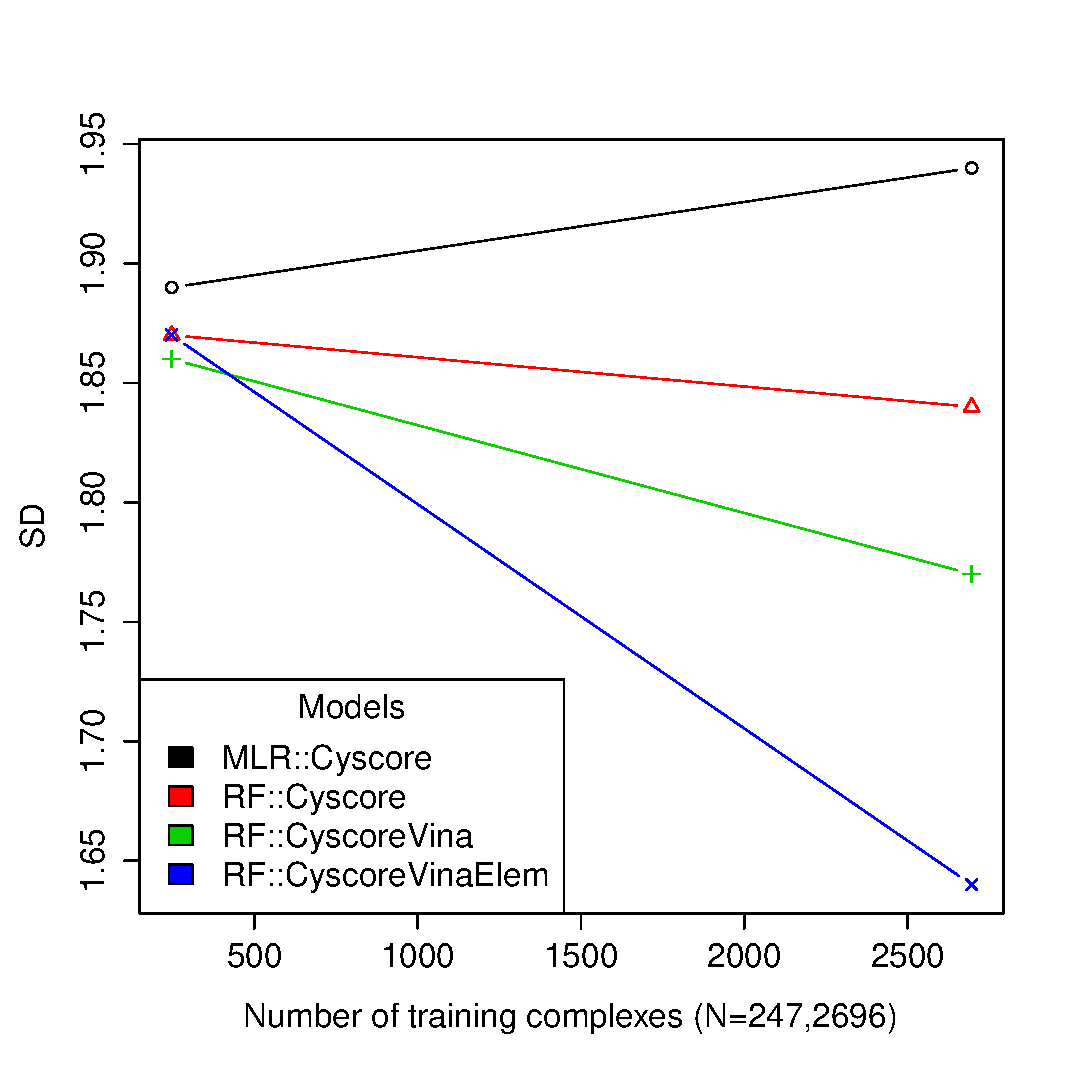
\includegraphics[width=\linewidth]{../rfcyscore/tst-201-sdev.eps}
\endminipage
\minipage{0.30\textwidth}
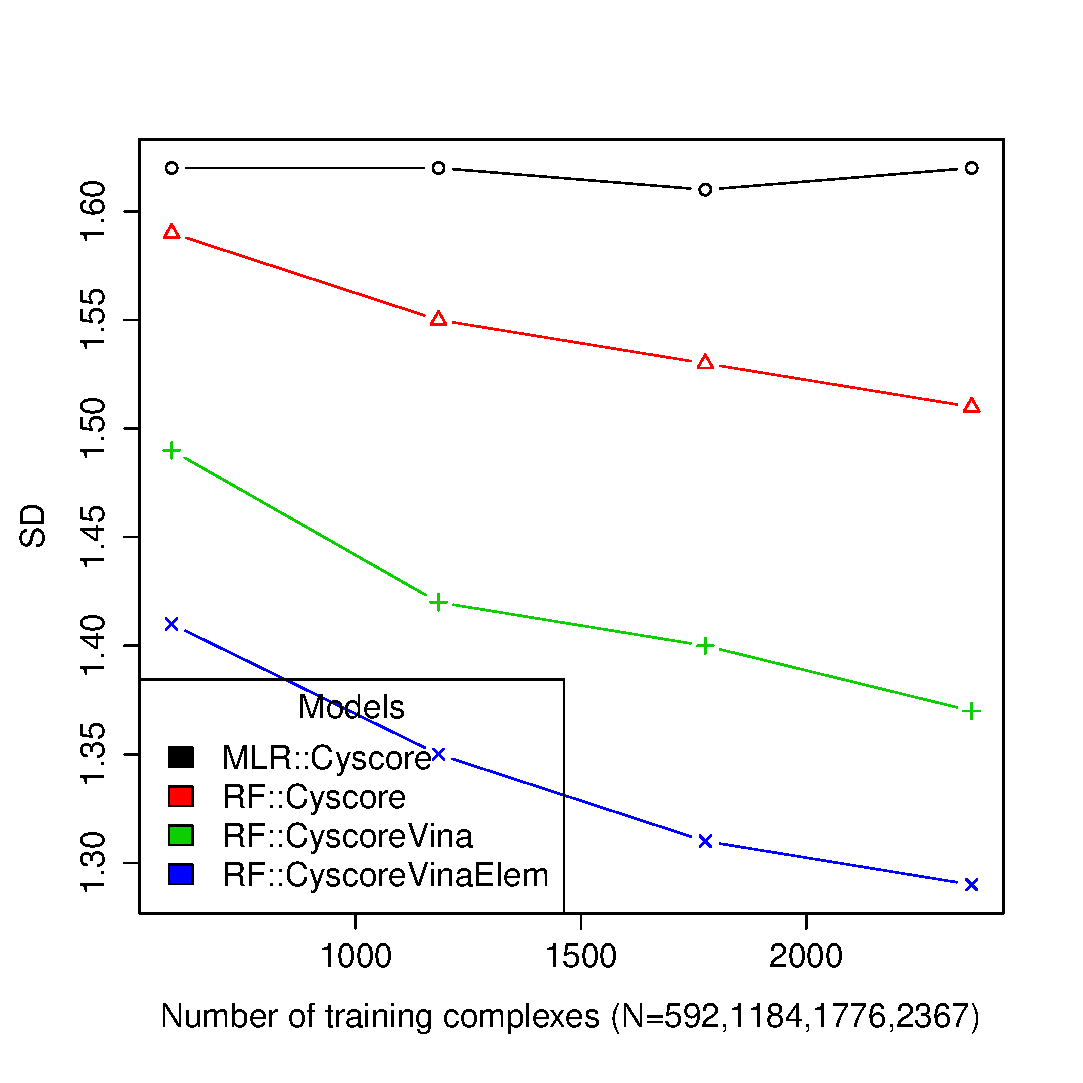
\includegraphics[width=\linewidth]{../rfcyscore/tst-592-sdev.eps}
\endminipage
\\
\minipage{0.30\textwidth}
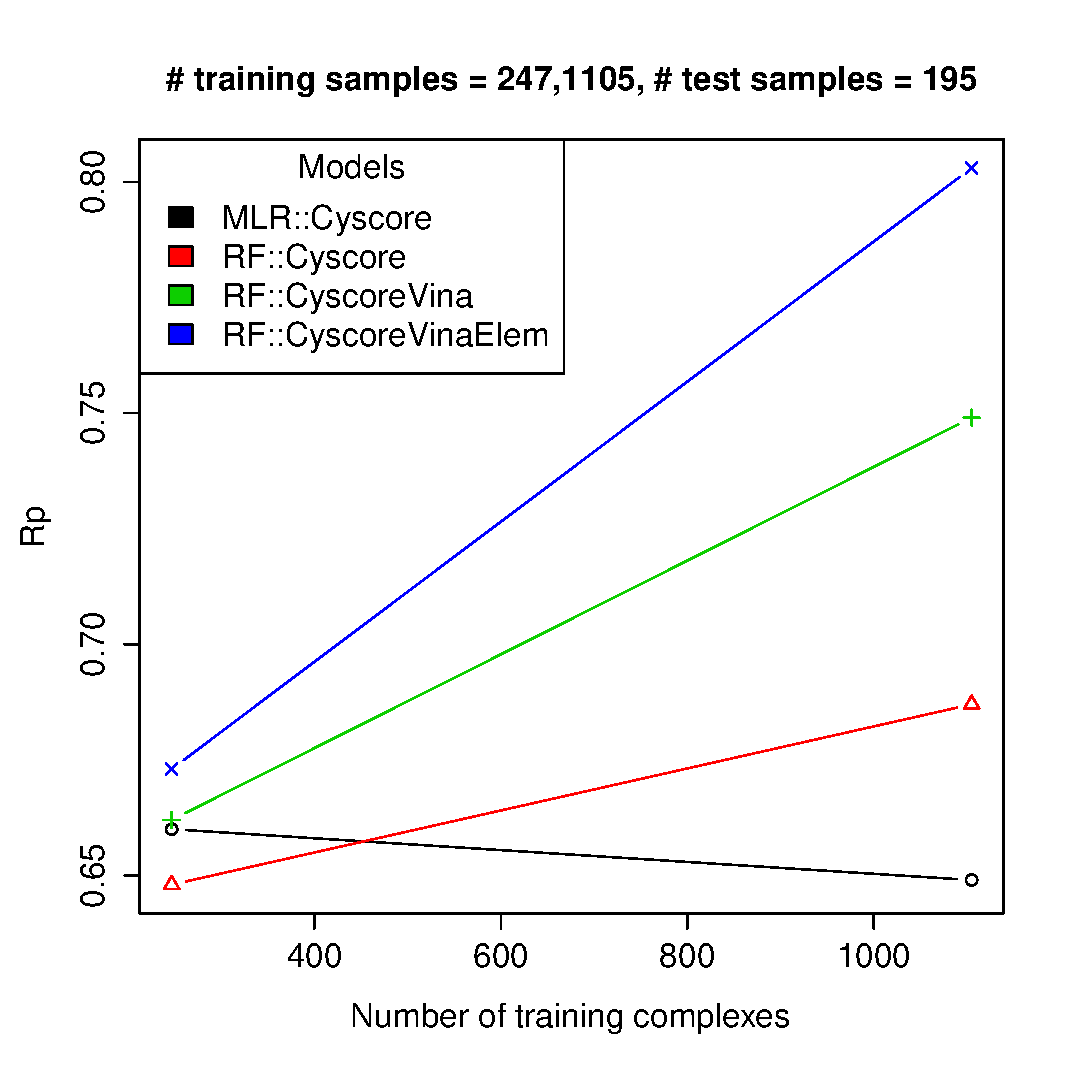
\includegraphics[width=\linewidth]{../rfcyscore/tst-195-pcor.eps}
\endminipage
\minipage{0.30\textwidth}
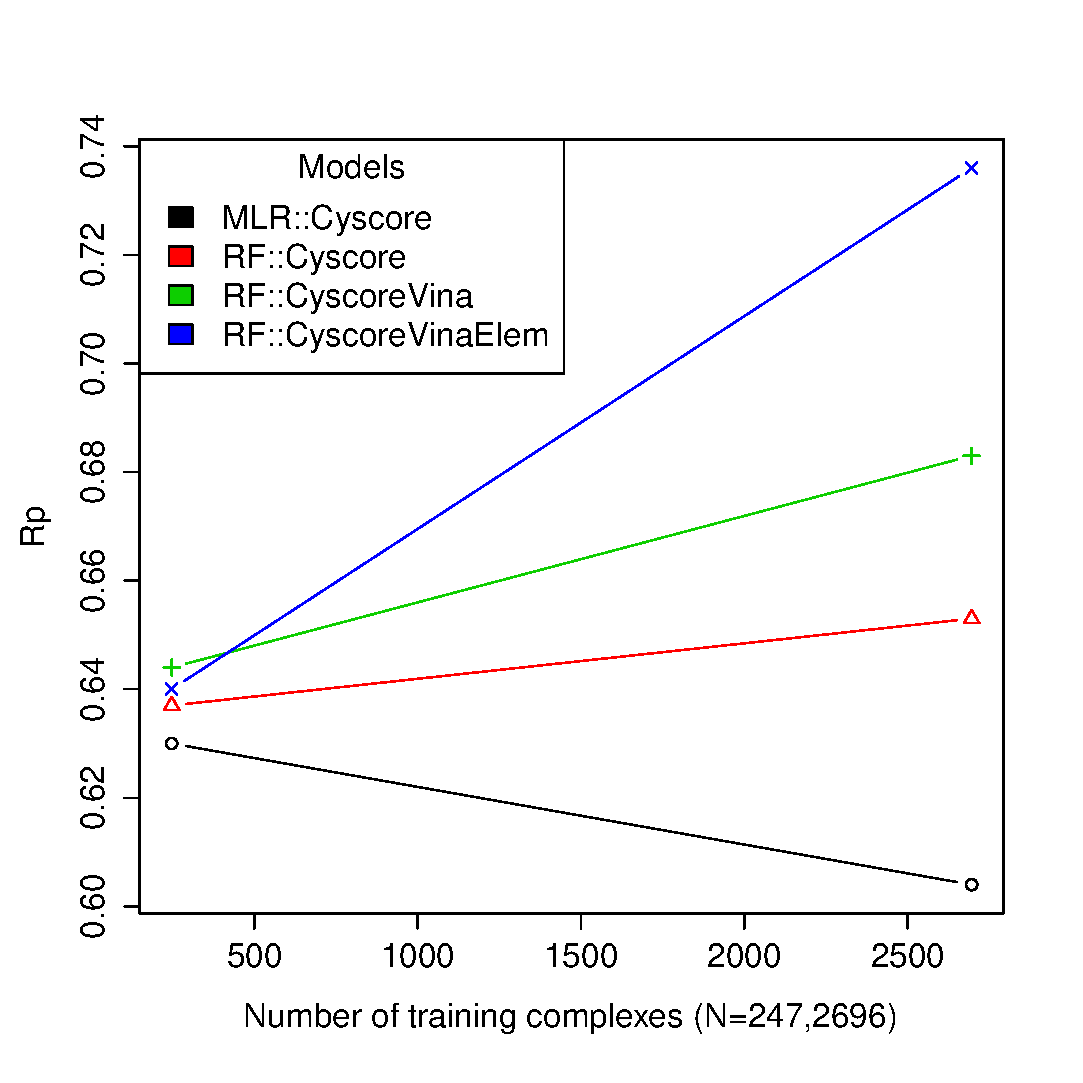
\includegraphics[width=\linewidth]{../rfcyscore/tst-201-pcor.eps}
\endminipage
\minipage{0.30\textwidth}
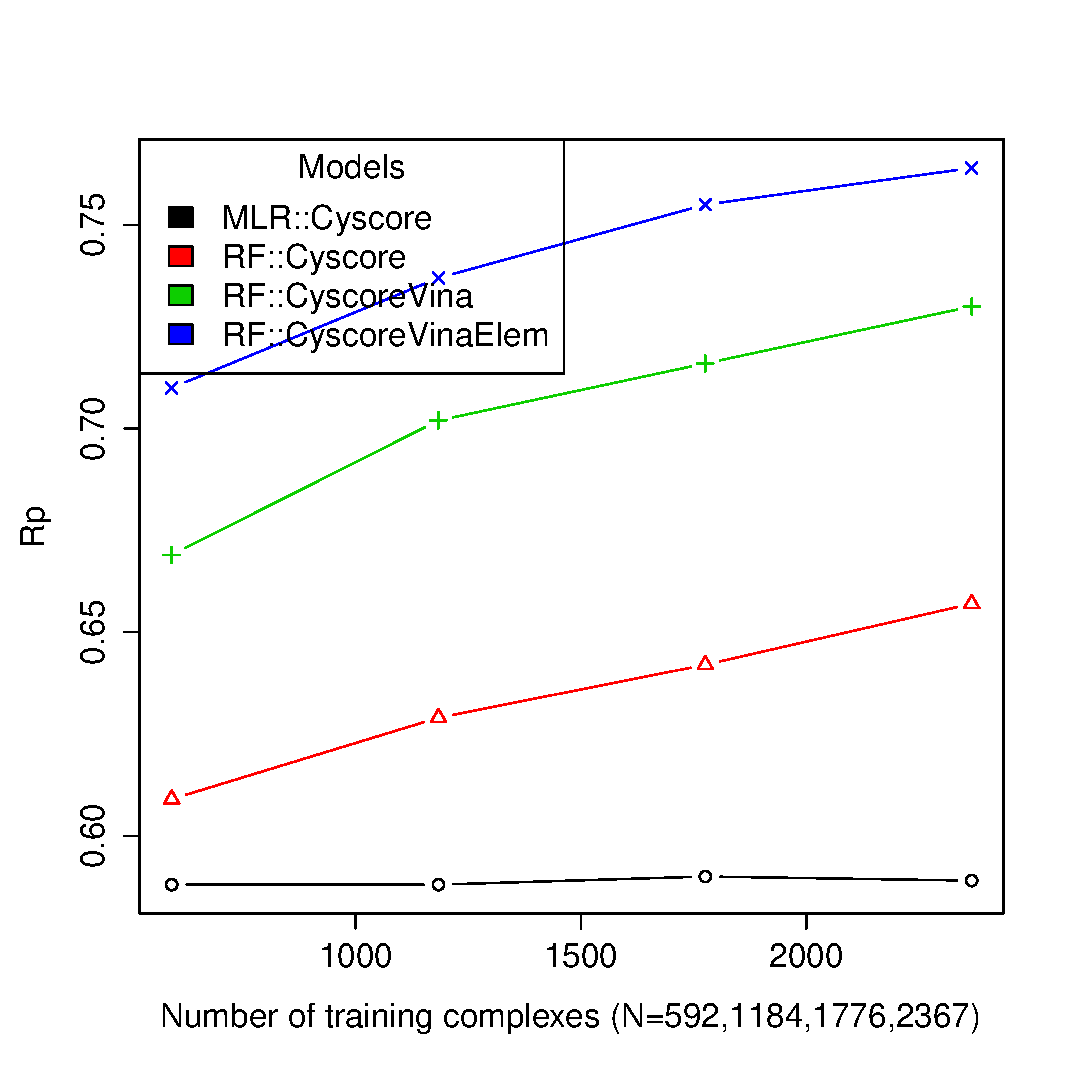
\includegraphics[width=\linewidth]{../rfcyscore/tst-592-pcor.eps}
\endminipage
\\
\minipage{0.30\textwidth}
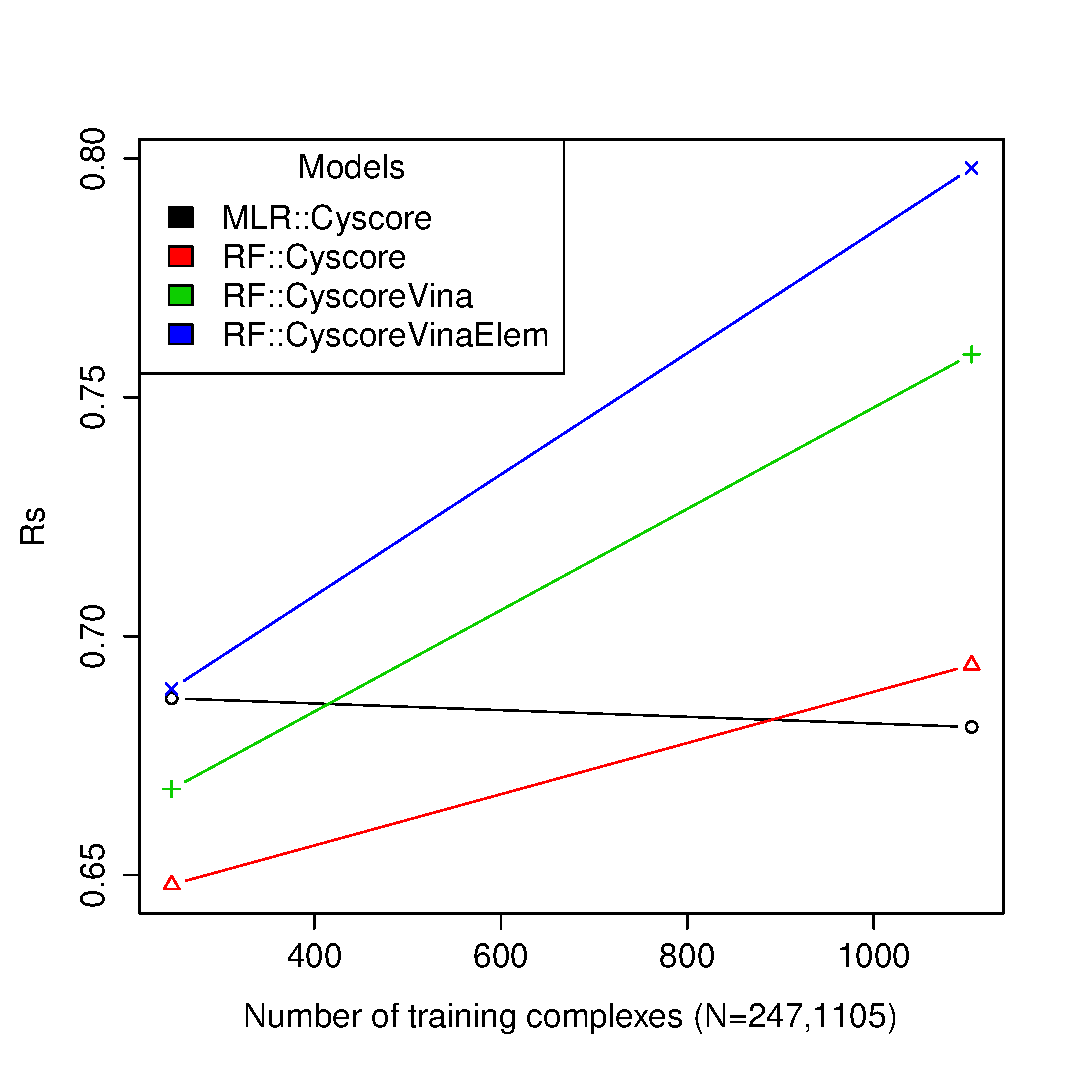
\includegraphics[width=\linewidth]{../rfcyscore/tst-195-scor.eps}
\endminipage
\minipage{0.30\textwidth}
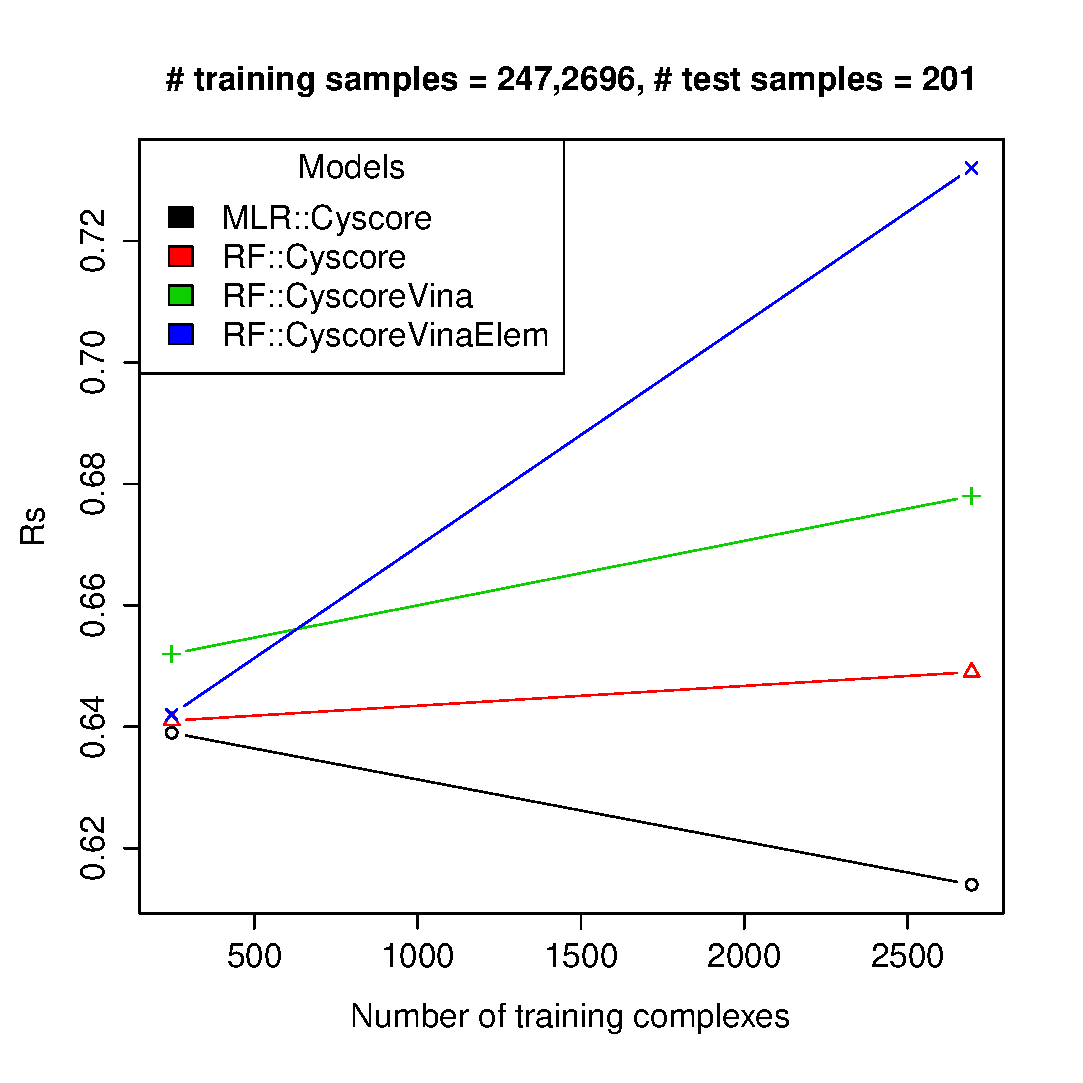
\includegraphics[width=\linewidth]{../rfcyscore/tst-201-scor.eps}
\endminipage
\minipage{0.30\textwidth}
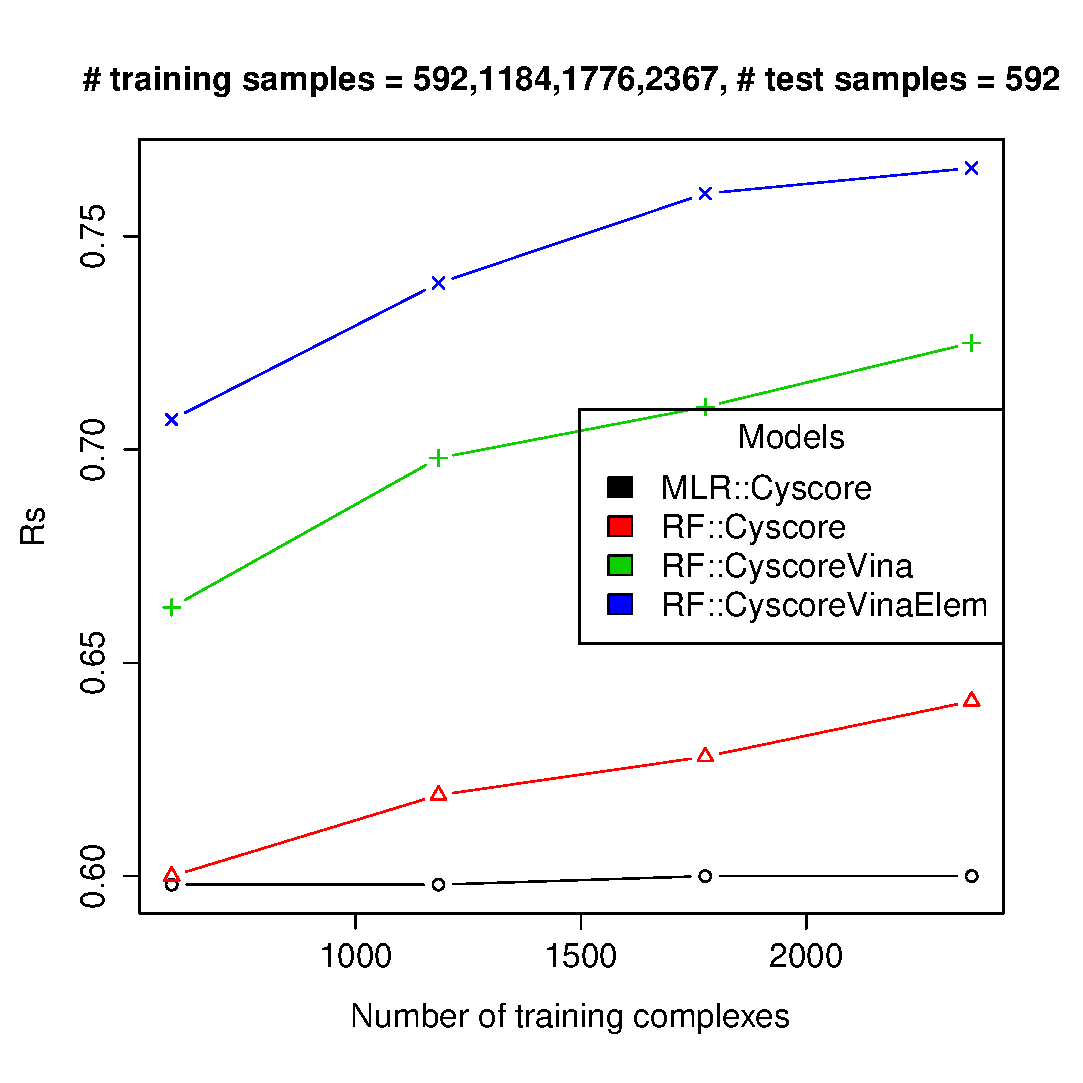
\includegraphics[width=\linewidth]{../rfcyscore/tst-592-scor.eps}
\endminipage
\caption{Prediction performance of regression models MLR and RF trained with varying numbers of features and samples. Left: PDBbind v2007 benchmark (N=195). Center: PDBbind v2012 benchmark (N=201). Right: PDBbind v2013 benchmark (N=592).}
\label{fig:stat}
\end{figure}

\subsection{MLR performance does not increase with more training samples}

On both PDBbind v2007 and v2012 benchmarks, MLR performed best when it was trained on the 247 carefully selected complexes as used by Cyscore. Its performance dropped when more complexes were used for training. On PDBbind v2013 benchmark, MLR performance stayed flat regardless of training sample sizes.

These results show that MLR is unable to exploit large sizes of structural data given only a small set of sophisticated features. Feeding more training samples to MLR actually increases the difficulty in regressing the coefficients well. Generally it would be a good idea to select fewer but high quality samples to train MLR, as was the case of Cyscore.

\subsection{RF requires sufficient structural features and training samples to comprehensively learn knowledge}

On all three benchmarks, given the same structural features, the RF models trained with more samples resulted in higher prediction accuracy. Similarly, given the same training samples, the RF models trained with more structural features resulted in higher prediction accuracy.

These results suggest that RF is capable of effectively exploiting a comprehensive set of structural features and training samples. Generally the more training samples, the more knowledge for RF to learn so as to capture the non-linearity of the structural data. Likewise, the more appropriate features, the higher probability of choosing the best splitting feature that can result in a high purity gain at non-leaf nodes during RF construction, and hence the higher chance of boosted RF performance.

\subsection{RF performs consistently well in cross validation}

Table \ref{tbl:cv} shows the results of the 5-fold cross validation. For all the four models, the best performance was obtained on partition 2. In terms of average performance, the relative performance ranking is consistent, where RF::CyscoreVinaElem (RMSE=1.35, SD=1.35, Rp=0.738, Rs=0.738) is better than RF::CyscoreVina (RMSE=1.44, SD=1.44, Rp=0.693, Rs=0.690), which is better than RF::Cyscore (RMSE=1.59, SD=1.59, Rp=0.603, Rs=0.587), which is better than MLR::Cyscore (RMSE=1.66, SD=1.66, Rp=0.556, Rs=0.559).

\begin{table}
\caption{Cross validation results of the four models on the five partitions of PDBbind v2013 refined set (N=2959).}
\label{tbl:cv}
\begin{tabular}{rrrrr}
\hline
\# & RMSE & SD & Rp & Rs\\
\hline
\multicolumn{5}{l}{MLR::Cyscore}\\
  1 & 1.66 & 1.66 & 0.560 & 0.555\\
  2 & 1.62 & 1.62 & 0.589 & 0.600\\
  3 & 1.69 & 1.70 & 0.531 & 0.529\\
  4 & 1.68 & 1.68 & 0.542 & 0.557\\
  5 & 1.65 & 1.65 & 0.559 & 0.553\\
avg & 1.66 & 1.66 & 0.556 & 0.559\\
\hline
\multicolumn{5}{l}{RF::Cyscore}\\
  1 & 1.60 & 1.60 & 0.601 & 0.588\\
  2 & 1.51 & 1.51 & 0.657 & 0.641\\
  3 & 1.66 & 1.66 & 0.561 & 0.545\\
  4 & 1.63 & 1.63 & 0.580 & 0.576\\
  5 & 1.57 & 1.57 & 0.615 & 0.586\\
avg & 1.59 & 1.59 & 0.603 & 0.587\\
\hline
\multicolumn{5}{l}{RF::CyscoreVina}\\
  1 & 1.41 & 1.41 & 0.708 & 0.709\\
  2 & 1.38 & 1.37 & 0.730 & 0.725\\
  3 & 1.49 & 1.49 & 0.668 & 0.665\\
  4 & 1.51 & 1.51 & 0.657 & 0.661\\
  5 & 1.42 & 1.42 & 0.701 & 0.692\\
avg & 1.44 & 1.44 & 0.693 & 0.690\\
\hline
\multicolumn{5}{l}{RF::CyscoreVinaElem}\\
  1 & 1.33 & 1.33 & 0.748 & 0.746\\
  2 & 1.30 & 1.29 & 0.764 & 0.766\\
  3 & 1.41 & 1.41 & 0.711 & 0.709\\
  4 & 1.41 & 1.41 & 0.711 & 0.722\\
  5 & 1.30 & 1.30 & 0.758 & 0.749\\
avg & 1.35 & 1.35 & 0.738 & 0.738\\
\hline
\end{tabular}
\end{table}

\subsection{Machine-learning scoring functions are significantly more accurate than empirical scoring functions}

Table \ref{tbl:trn1105tst195} compares Cyscore, RF::Cyscore, RF::CyscoreVina and RF::CyscoreVinaElem against 20 other scoring functions on PDBbind v2007 core set (N=195), with RF::CyscoreVinaElem performing best in terms of Rp, Rs and SD.

\begin{table}[ht]
\caption{Prediction performance of 24 scoring functions evaluated on PDBbind v2007 core set (N=195) in terms of Pearson correlation coefficient Rp, Spearman correlation coefficient Rs and standard deviation SD in linear correlation on the test set. The scoring functions are sorted in the descending order of Rp. RF::CyscoreVinaElem and Cyscore rank 1st and 8th respectively in terms of Rp. The statistics for the other 20 scoring functions are collected from \cite{1362,1370}.}
\label{tbl:trn1105tst195}
\begin{tabular}{lrrr}
\hline
Scoring function & Rp & Rs & SD\\
\hline
RF::CyscoreVinaElem & 0.803 & 0.798 & 1.42\\
RF-Score::Elem-v2 & 0.803 & 0.797 & 1.54 \\
RF-Score & 0.774 & 0.762 & 1.59\\
ID-Score & 0.753 & 0.779 & 1.63\\
RF::CyscoreVina & 0.749 & 0.759 & 1.58\\
SVR-Score & 0.726 & 0.739 & 1.70\\
RF::Cyscore & 0.687 & 0.694 & 1.73\\
Cyscore & 0.660 & 0.687 & 1.79\\
X-Score::HMScore & 0.644 & 0.705 & 1.83\\
DrugScoreCSD & 0.569 & 0.627 & 1.96\\
SYBYL::ChemScore & 0.555 & 0.585 & 1.98\\
DS::PLP1 & 0.545 & 0.588 & 2.00\\
GOLD::ASP & 0.534 & 0.577 & 2.02\\
SYBYL::G-Score & 0.492 & 0.536 & 2.08\\
DS::LUDI3 & 0.487 & 0.478 & 2.09\\
DS::LigScore2 & 0.464 & 0.507 & 2.12\\
GlideScore-XP & 0.457 & 0.435 & 2.14\\
DS::PMF & 0.445 & 0.448 & 2.14\\
GOLD::ChemScore & 0.441 & 0.452 & 2.15\\
SYBYL::D-Score & 0.392 & 0.447 & 2.19\\
DS::Jain & 0.316 & 0.346 & 2.24\\
GOLD::GoldScore & 0.295 & 0.322 & 2.29\\
SYBYL::PMF-Score & 0.268 & 0.273 & 2.29\\
SYBYL::F-Score & 0.216 & 0.243 & 2.35\\
\hline
\end{tabular}
\end{table}

\subsection{Substituting RF for MLR strongly improves Cyscore}

Figure \ref{fig:cor} compares the prediction performance of Cyscore and RF::CyscoreVinaElem, with RF::CyscoreVinaElem improving Cyscore by -0.28 in RMSE, -0.37 in SD, +0.143 in Rp and +0.111 in Rs on the PDBbind v2007 benchmark, by -0.14 in RMSE, -0.25 in SD, +0.106 in Rp and +0.093 in Rs on the PDBbind v2012 benchmark, and by -0.40 in RMSE, -0.29 in SD, +0.187 in Rp and +0.184 in Rs on the PDBbind v2013 benchmark.

\begin{figure}[ht!]
\minipage{0.33\textwidth}
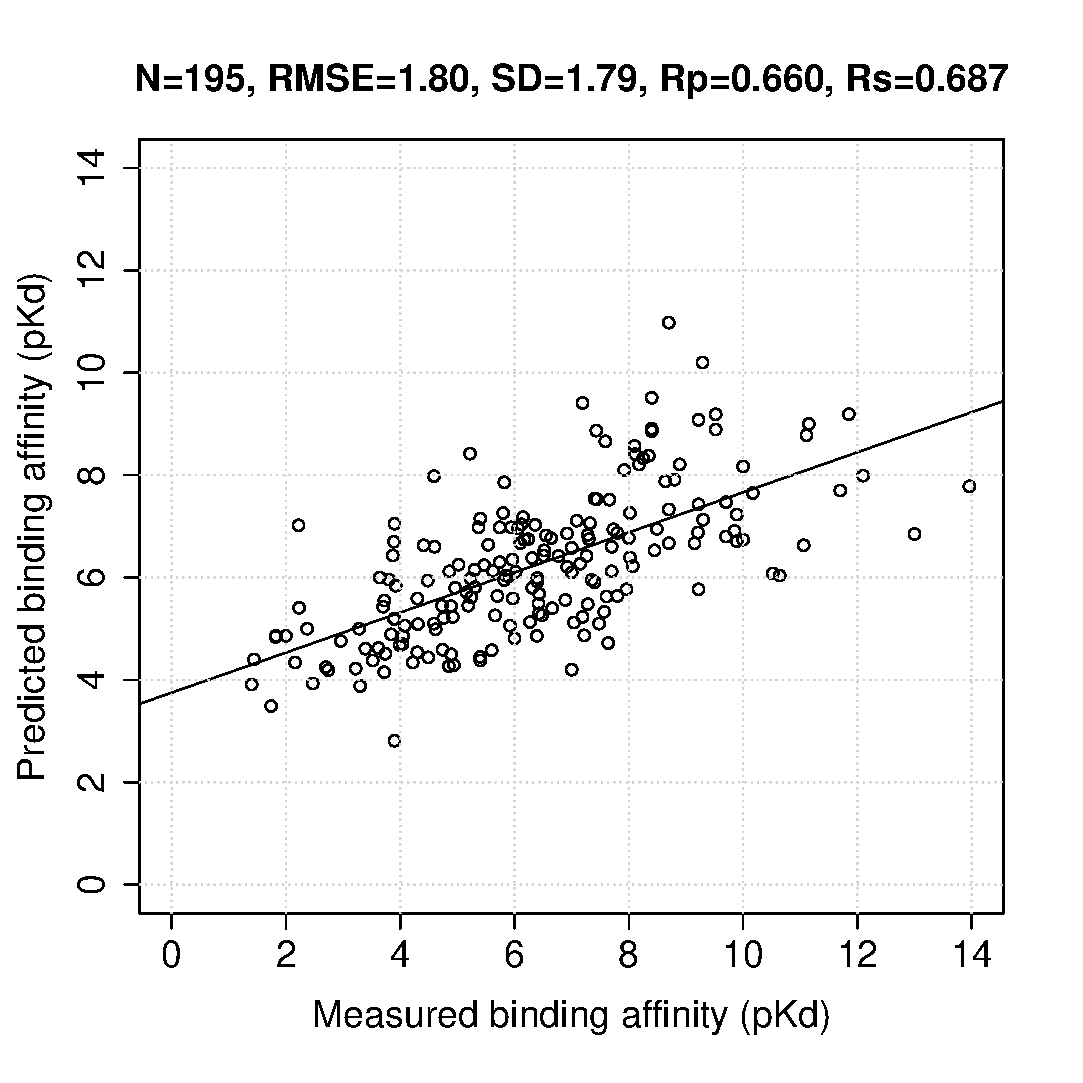
\includegraphics[width=\linewidth]{../rfcyscore/x4/mlr/trn-247-tst-195-yp.eps}
\endminipage
\minipage{0.33\textwidth}
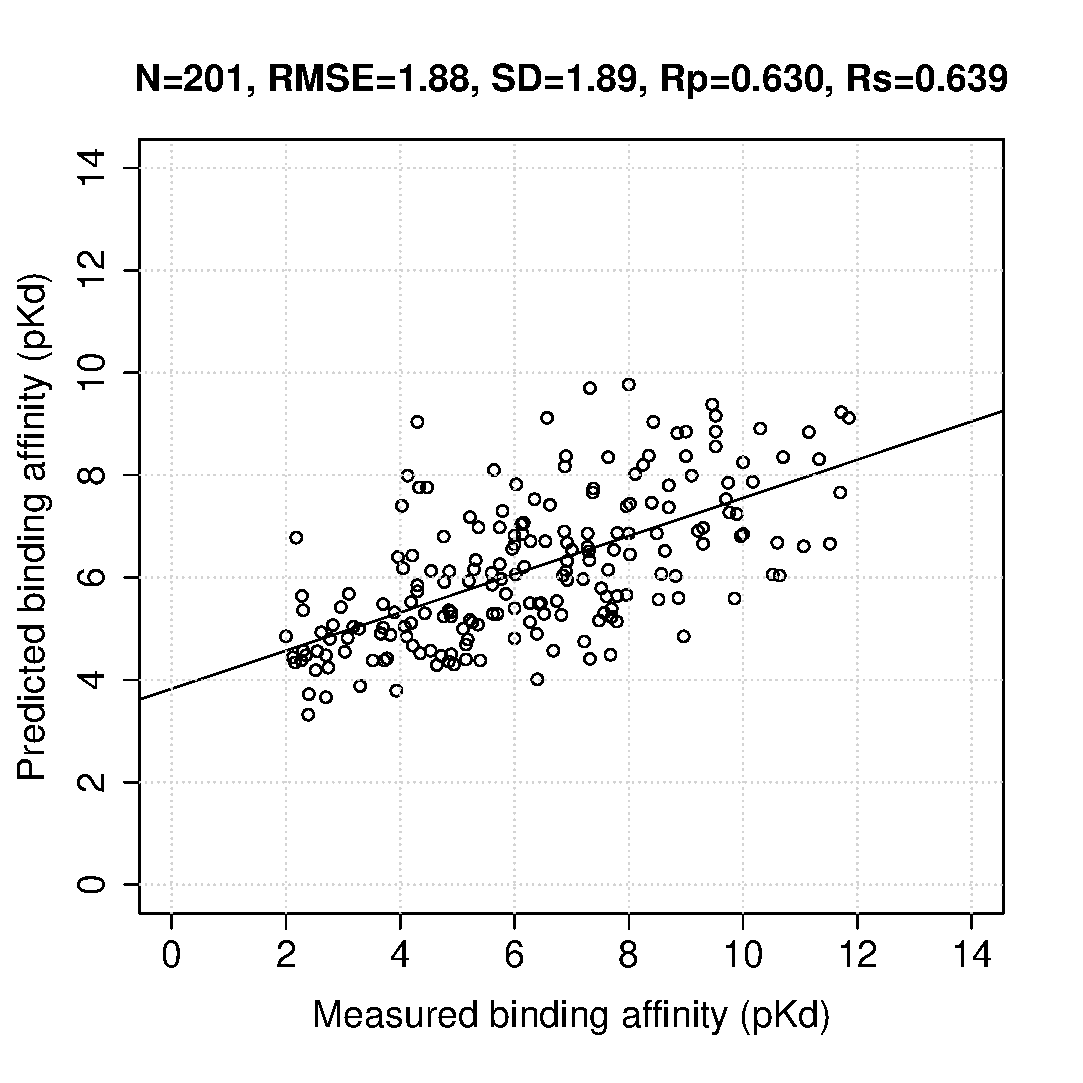
\includegraphics[width=\linewidth]{../rfcyscore/x4/mlr/trn-247-tst-201-yp.eps}
\endminipage
\minipage{0.33\textwidth}
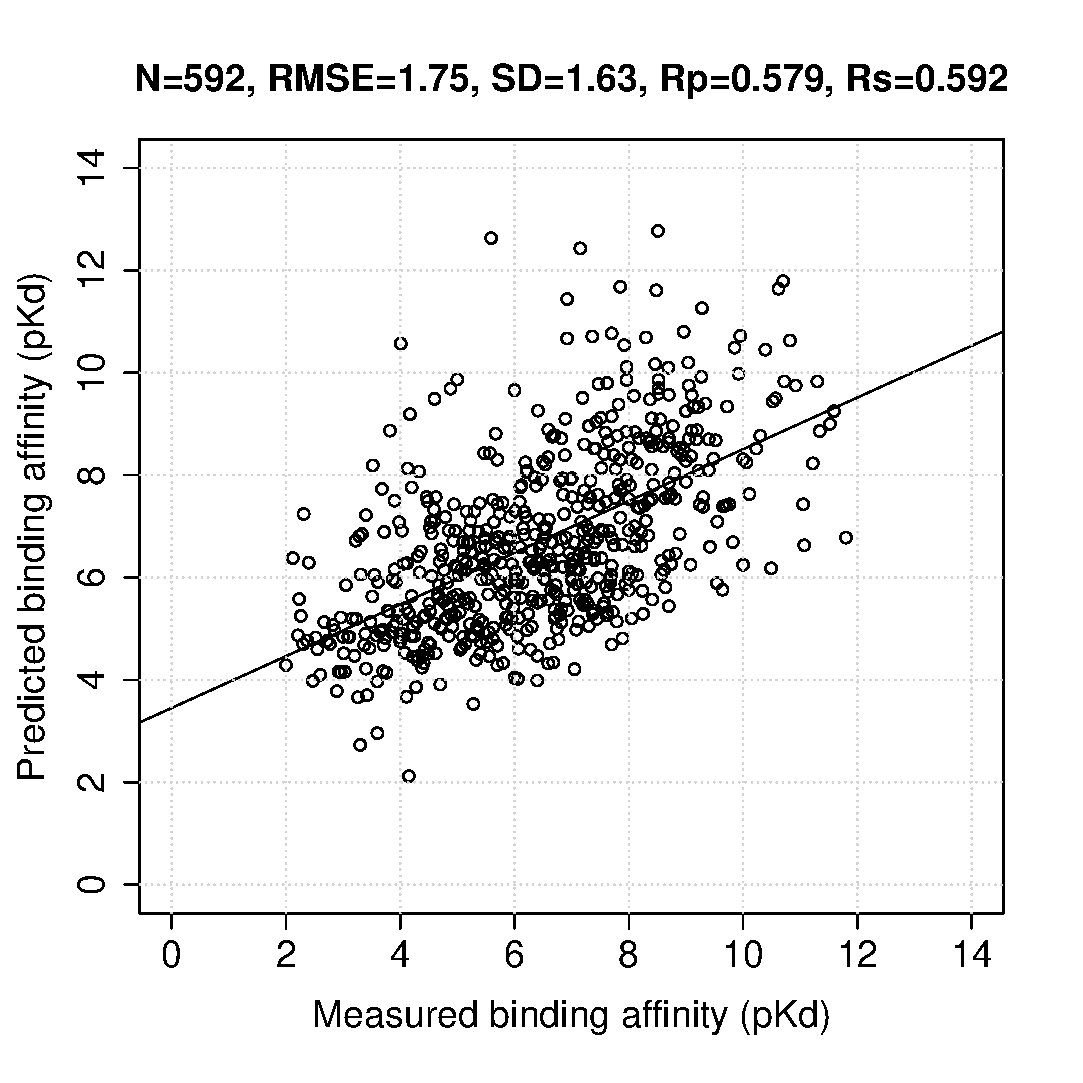
\includegraphics[width=\linewidth]{../rfcyscore/x4/mlr/trn-247-tst-592-yp.eps}
\endminipage
\\
\minipage{0.33\textwidth}
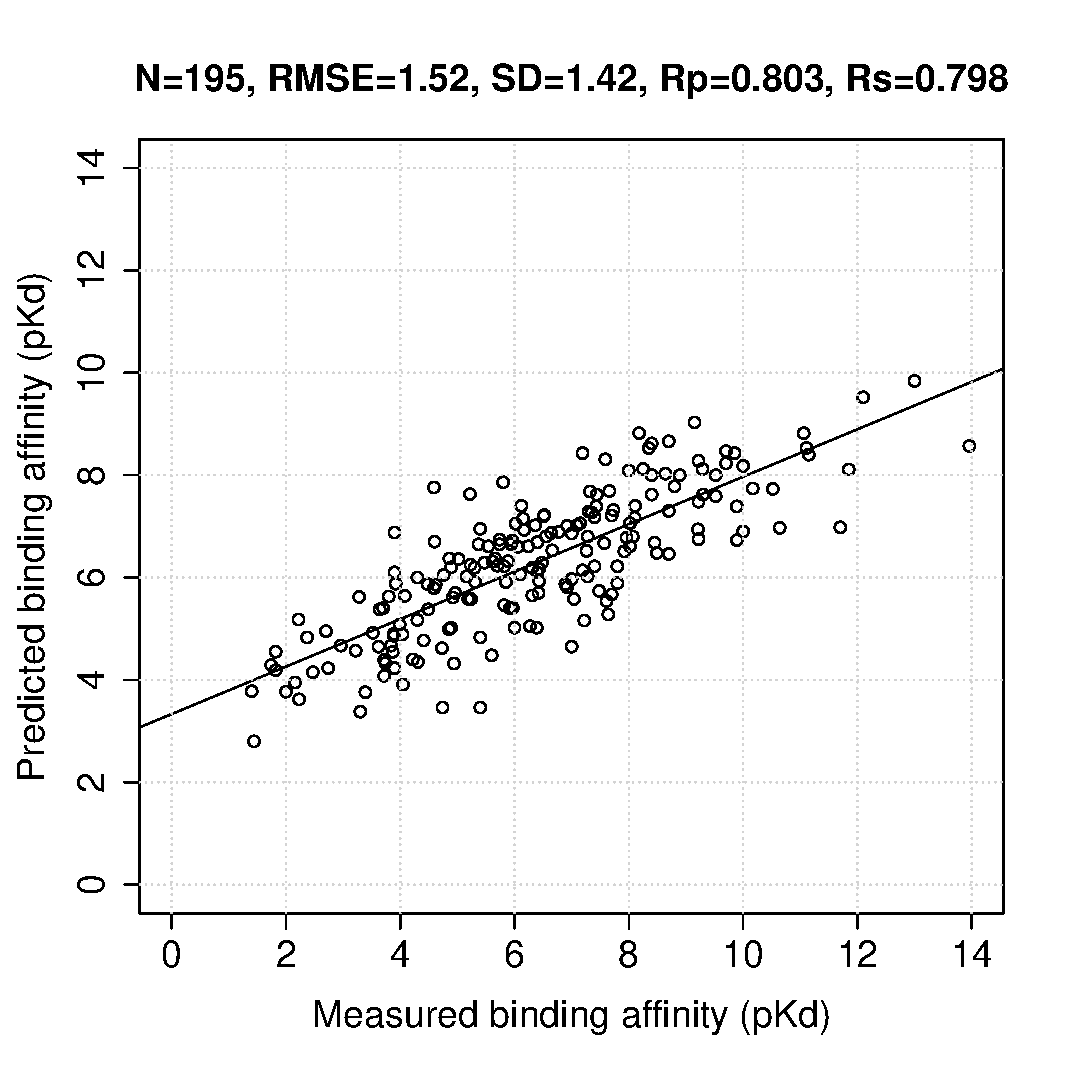
\includegraphics[width=\linewidth]{../rfcyscore/x46/rf/trn-1105-tst-195-yp.eps}
\endminipage
\minipage{0.33\textwidth}
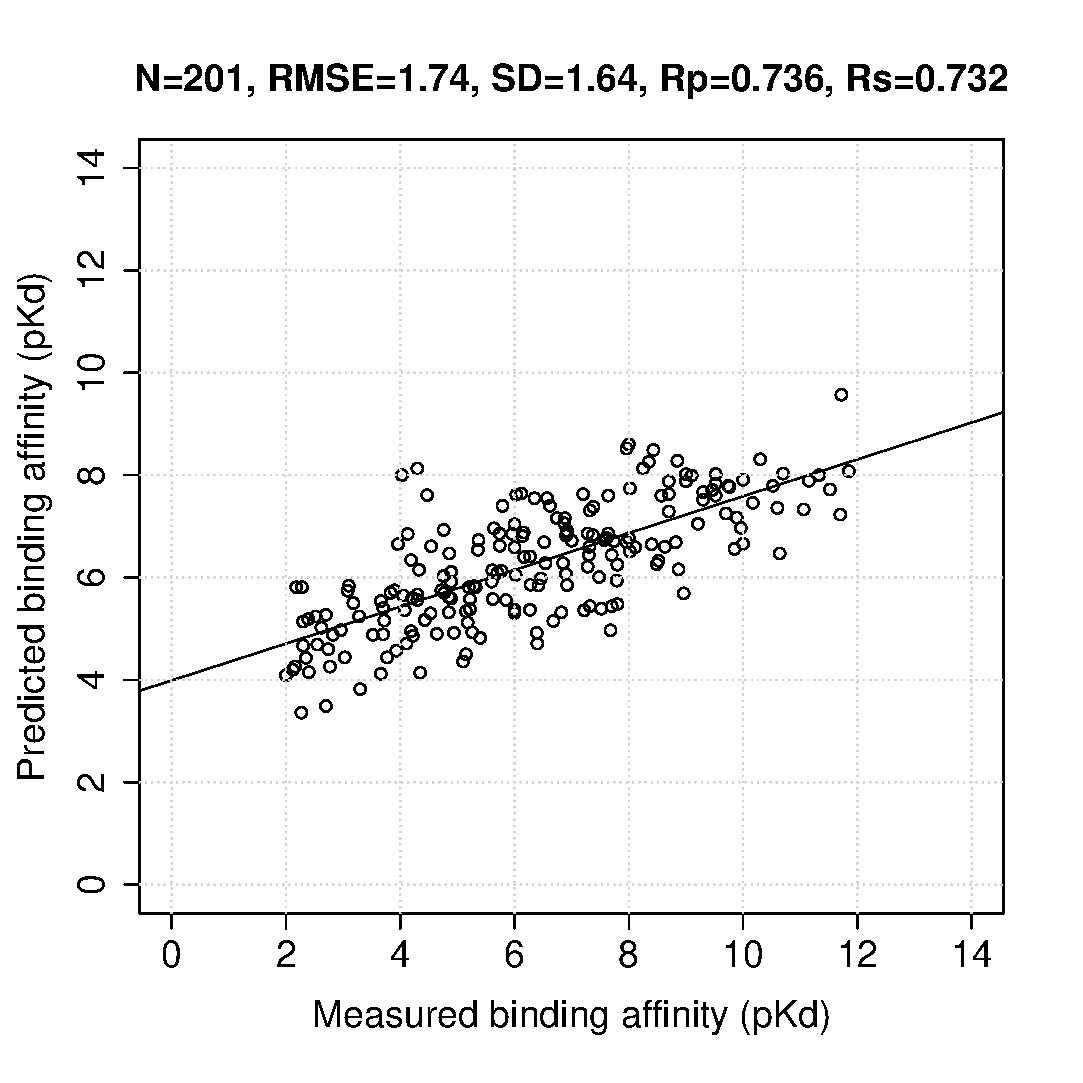
\includegraphics[width=\linewidth]{../rfcyscore/x46/rf/trn-2696-tst-201-yp.eps}
\endminipage
\minipage{0.33\textwidth}
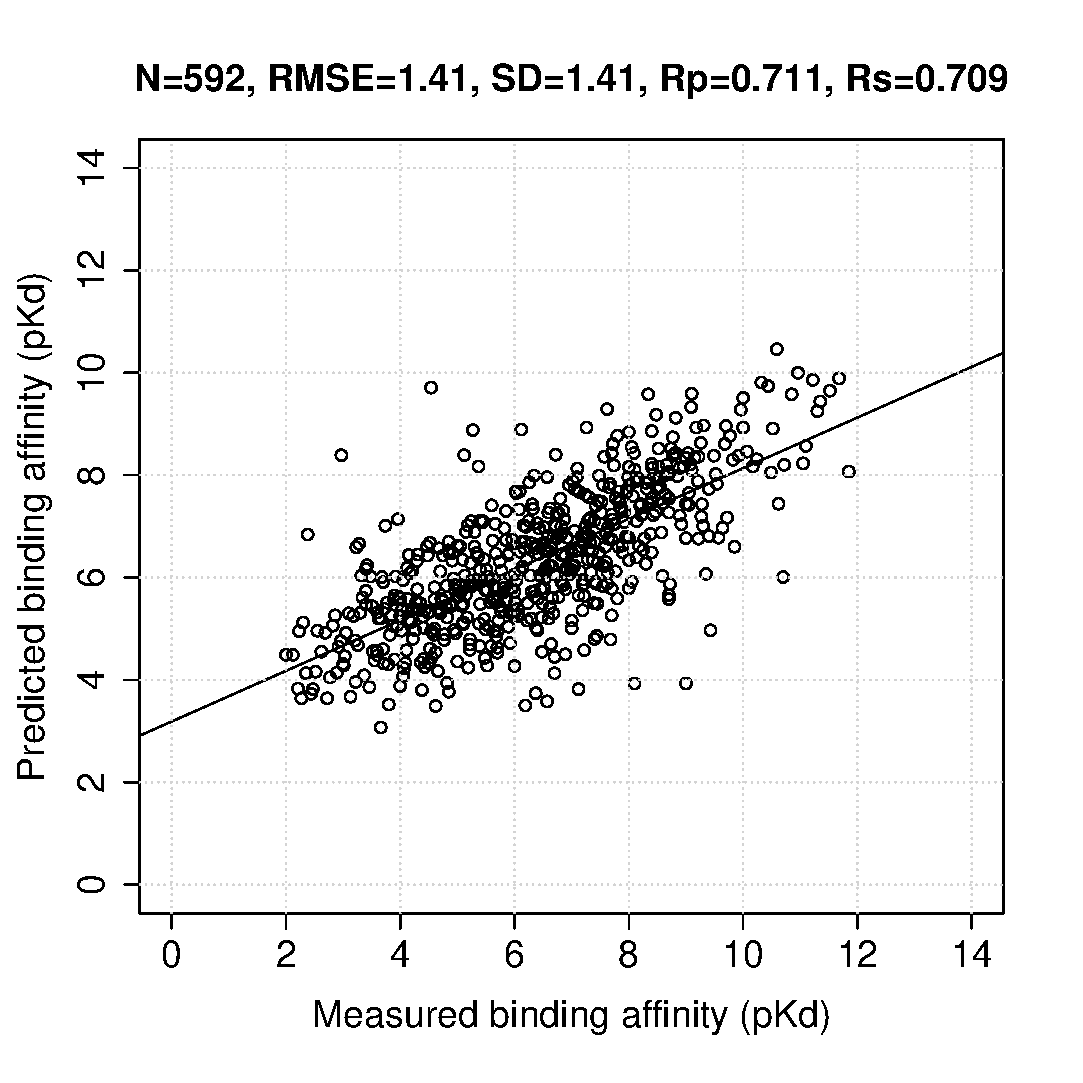
\includegraphics[width=\linewidth]{../rfcyscore/x46/rf/trn-2367-tst-592-yp.eps}
\endminipage
\caption{Correlation plots of predicted binding affinities against measured ones. Top: Cyscore. Bottom: RF::CyscoreVinaElem. Left: PDBbind v2007 benchmark (N=195), with RF::CyscoreVinaElem trained on 1105 complexes. Center: PDBbind v2012 benchmark (N=201), with RF::CyscoreVinaElem trained on 2696 complexes. Right: PDBbind v2013 benchmark (N=592), with RF::CyscoreVinaElem trained on 2367 complexes.}
\label{fig:cor}
\end{figure}

These results show that RF::CyscoreVinaElem performed consistently better than Cyscore on all the three benchmarks. One can develop a much more accurate scoring function out of an existing empirical one simply by changing the regression model from MLR to RF.

\subsection{RF-based scoring functions can be as interpretable as empirical ones} % TODO: delete this section.

The functional form of empirical scoring functions is straightforward, while it is implicit in RF-based scoring functions. It is therefore natural to doubt the interpretability of the latter. Nevertheless, one can estimate the importance of each particular feature by randomly permuting its training values, and the feature leading to the largest variation in the predicted binding affinity on OOB data can be regarded as the most important.

Figure \ref{fig:varimp} plots the percentage of increase in mean square error (\%IncMSE) observed when each of the 4 Cyscore features used to train RF was noised up. All the 4 features turned out to be important (\%IncMSE\textgreater 20), with van der Waals interaction energy and hydrophobic free energy being particularly important (\%IncMSE\textgreater 40). Correctly estimating variable importance can assist in a priori feature selection and in understanding ligand binding.

\begin{figure}
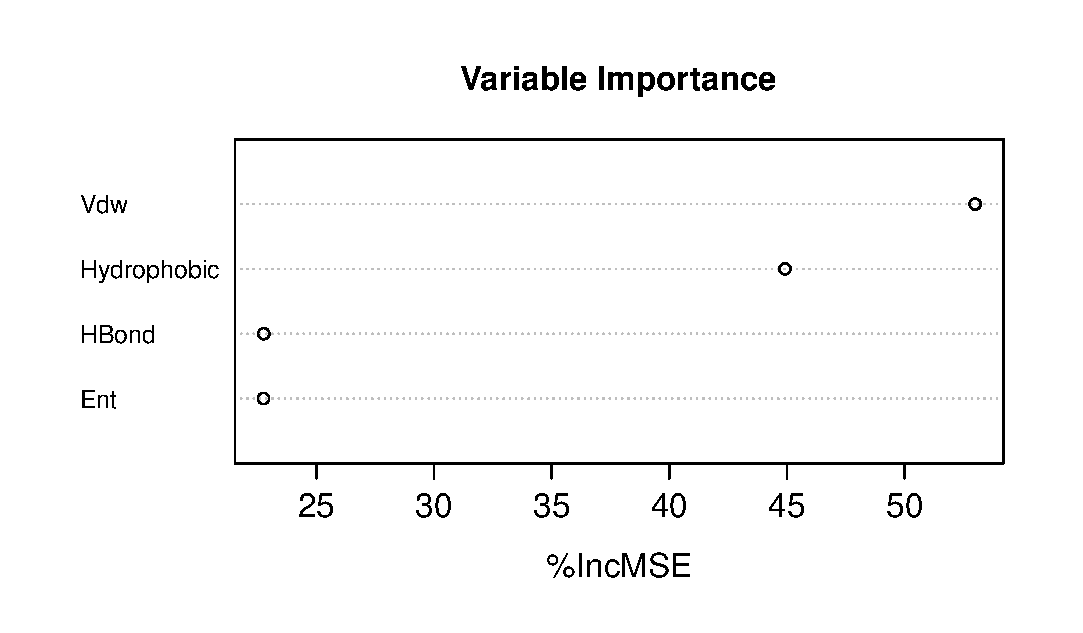
\includegraphics[width=\linewidth]{../rfcyscore/x4/rf/trn-1105.eps}
\caption{Feature importance estimated on internal OOB data of the 1105 complexes from PDBbind v2007 refined set. The \%IncMSE value of a particular feature was computed as the percentage of increase in mean square error observed in OOB prediction when that features was randomly permuted.}
\label{fig:varimp}
\end{figure}

\section{Conclusions}

Machine-learning scoring functions are fundamentally different from empirical ones because of circumventing the functional form on the relationship between structural features and binding affinities. In this study we have demonstrated that the multiple linear regression (MLR) model used in empirical scoring functions like Cyscore does not improve its performance in the presence of abundant training samples. When there are sufficient structural features and sufficient training samples, RF demonstrates its advantage over MLR by a large margin in comprehensively capturing the non-linear nature in the data. Under this circumstance, RF-based scoring functions assimilate data significantly better than empirical scoring functions. Improvements with dataset size can only be gained with the appropriate regression model anyway. Simply changing the regression model of Cyscore from MLR to RF and expanding the feature set and the sample set can significantly increase the prediction accuracy. The performance gap between MLR and RF will be further widened given the future availability of more and more resolved structures.

Moreover, empirical scoring functions usually rely on complicated energetic contributions that must be carefully devised from intermolecular interactions, whereas RF-based scoring functions can also effectively exploit features as simple as occurrence count of intermolecular contacts. In this study we have shown that using more structural features appropriately can also substantially enhance the prediction accuracy of RF. This further stresses the importance of substituting RF for MLR in scoring function development.

Last but not the least, RF-based scoring functions, having correctly estimated the feature importance, can be as interpretable as empirical ones.

%%%%%%%%%%%%%%%%%%%%%%%%%%%%%%%%%%%%%%%%%%%%%%%%%%%%%%%%%%%%%%%%%%%%%
%% The "Acknowledgement" section can be given in all manuscript
%% classes.  This should be given within the "acknowledgement"
%% environment, which will make the correct section or running title.
%%%%%%%%%%%%%%%%%%%%%%%%%%%%%%%%%%%%%%%%%%%%%%%%%%%%%%%%%%%%%%%%%%%%%
\begin{acknowledgement}

We gratefully acknowledge the Direct Grant from the Chinese University of Hong Kong, the GRF Grant (Project No. 2150764) from the Research Grants Council of Hong Kong SAR, and the Medical Research Council for a Methodology Research Fellowship (Grant No. G0902106, awarded to P.J.B.). We thank Yang Cao for helping us to reproduce the Cyscore results.

\end{acknowledgement}

%%%%%%%%%%%%%%%%%%%%%%%%%%%%%%%%%%%%%%%%%%%%%%%%%%%%%%%%%%%%%%%%%%%%%
%% The same is true for Supporting Information, which should use the
%% suppinfo environment.
%%%%%%%%%%%%%%%%%%%%%%%%%%%%%%%%%%%%%%%%%%%%%%%%%%%%%%%%%%%%%%%%%%%%%
\begin{suppinfo}

\paragraph{stat.xlsx} contains the prediction performance of regression models MLR and RF trained with varying numbers of features and samples and tested on the PDBbind v2007, v2012 and v2013 benchmarks in terms of root mean square error RMSE, standard deviation SD in linear correlation on the test set, Pearson correlation coefficient Rp and Spearman correlation coefficient Rs.

\paragraph{cv.xlsx} contains the PDB IDs and measured binding affinities of the protein-ligand complexes in the five partitions of PDBbind v2013 refined set.

\end{suppinfo}

%%%%%%%%%%%%%%%%%%%%%%%%%%%%%%%%%%%%%%%%%%%%%%%%%%%%%%%%%%%%%%%%%%%%%
%% The appropriate \bibliography command should be placed here.
%% Notice that the class file automatically sets \bibliographystyle
%% and also names the section correctly.
%%%%%%%%%%%%%%%%%%%%%%%%%%%%%%%%%%%%%%%%%%%%%%%%%%%%%%%%%%%%%%%%%%%%%
\bibliography{../refworks}

\end{document}

%Journal of Chemical Information and Modeling 4.304
%Journal of Cheminformatics 3.59
%BMC Bioinformatics 3.02
%Molecular Informatics 2.338

%Sheng-Yong Yang, yangsy@scu.edu.cn, State Key Laboratory of Biotherapy and Cancer Center, West China Hospital, West China Medical School, Sichuan University, Sichuan 610041, China
%Dik-Lung Ma, edmondma@hkbu.edu.hk, Department of Chemistry, Hong Kong Baptist University, Kowloon Tong, China
%Elizabeth Yuriev, Elizabeth.Yuriev@monash.edu, Medicinal Chemistry, Monash Institute of Pharmaceutical Sciences, Monash University, Parkville, VIC, Australia
%Samy O. Meroueh, smeroueh@iupui.edu, Department of Biochemistry and Molecular Biology, Indiana University, Indianapolis, Indiana, United States
%James B. Dunbar, Jr., jbdunbar@umich.edu, Department of Medicinal Chemistry, University of Michigan, 428 Church Street, Ann Arbor, Michigan 48109-1065, United States
